\chapter{Appendix}
\label{cha:appendx}

\begin{figure}[h]
     \centering
     \begin{subfigure}[b]{0.45\textwidth}
         \centering
         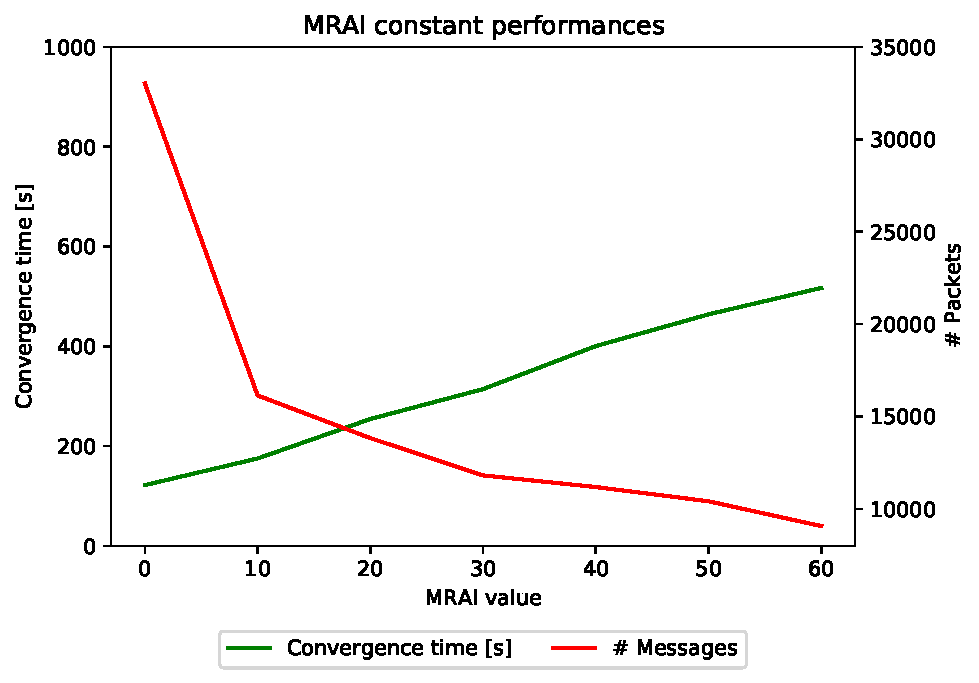
\includegraphics[width=\textwidth]{images/internet_like/1000/signals/AWAW/constant/internet_like-constant_AWAW_mrai_evolution.pdf}
		 \caption{Network perforcances, \textit{fixed} \ac{MRAI} strategy}
         \label{fig:internet_like_1000_fixed_AWAW}
     \end{subfigure}
     \hfill
     \begin{subfigure}[b]{0.45\textwidth}
         \centering
         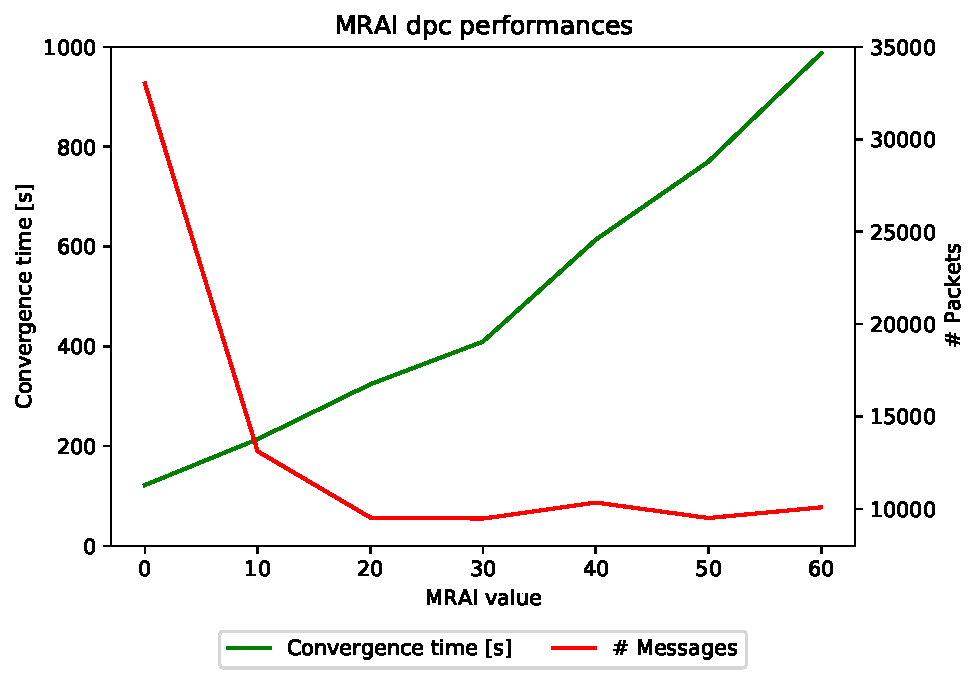
\includegraphics[width=\textwidth]{images/internet_like/1000/signals/AWAW/dpc/internet_like-DPC_AWAW_mrai_evolution.pdf}
		 \caption{Network perforcances, \ac{DPC} \ac{MRAI} strategy}
         \label{fig:internet_like_1000_dpc_AWAW}
     \end{subfigure}
	 \caption{Network perfomances comparison with different \ac{MRAI} strategies,
		Graph internet like with \num{1000} nodes, signal \q{AWAW}}
        \label{fig:internt_like_1000_evolution_AWAW}
\end{figure}

\begin{figure}[h]
     \centering
     \begin{subfigure}[b]{0.45\textwidth}
         \centering
         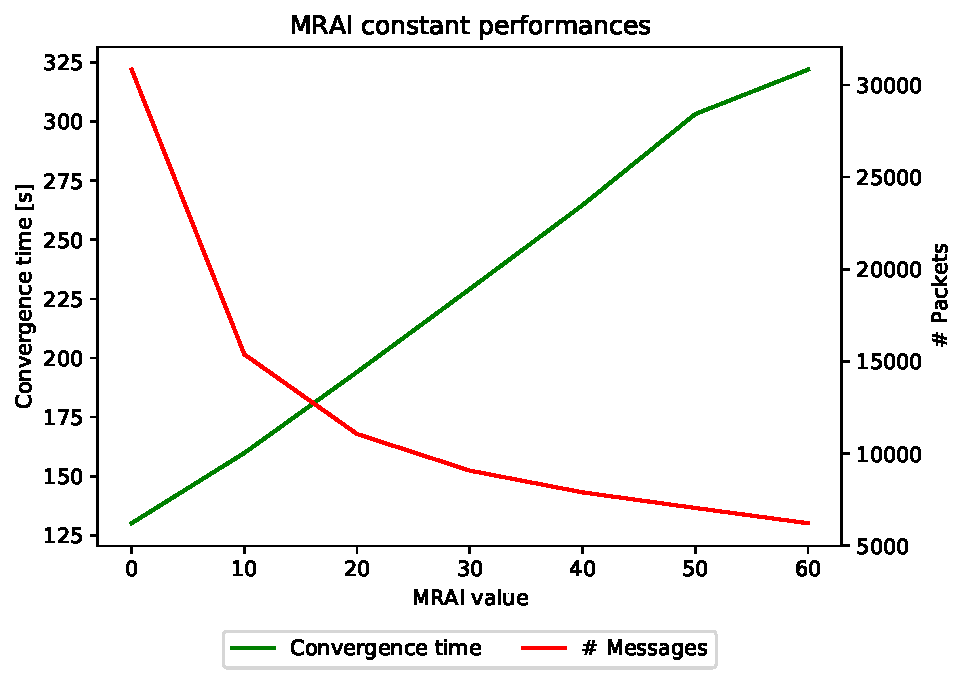
\includegraphics[width=\textwidth]{images/internet_like/1000/signals/AWAWA/constant/internet_like-constant_AWAWA_mrai_evolution.pdf}
		 \caption{Network perforcances, \textit{fixed} \ac{MRAI} strategy}
         \label{fig:internet_like_1000_fixed_AWAWA}
     \end{subfigure}
     \hfill
     \begin{subfigure}[b]{0.45\textwidth}
         \centering
         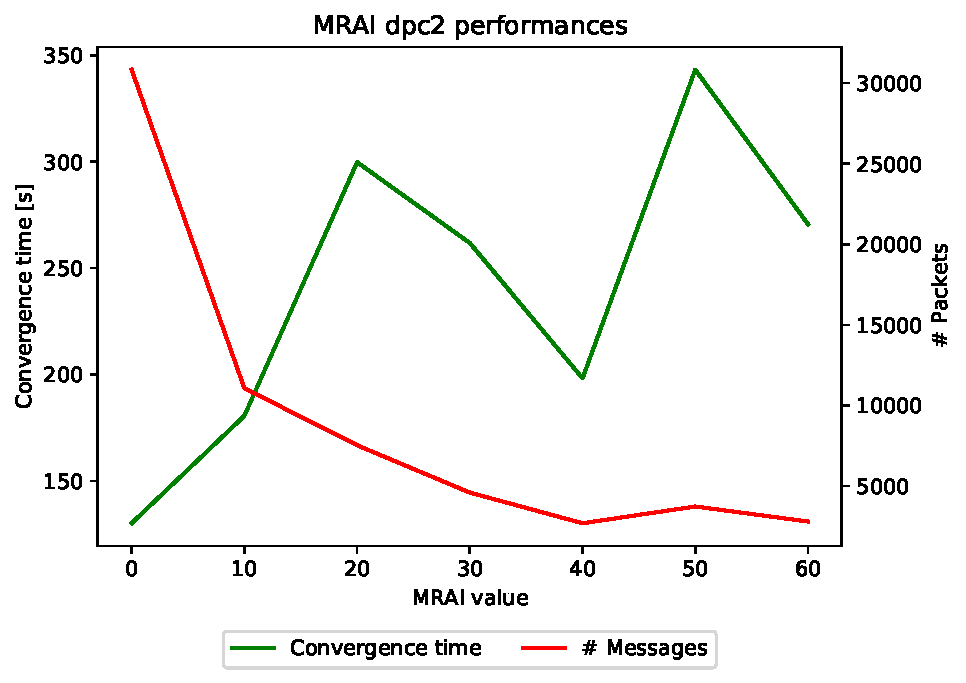
\includegraphics[width=\textwidth]{images/internet_like/1000/signals/AWAWA/dpc/internet_like-DPC_AWAWA_mrai_evolution.pdf}
		 \caption{Network perforcances, \ac{DPC} \ac{MRAI} strategy}
         \label{fig:internet_like_1000_dpc_AWAWA}
     \end{subfigure}
	 \caption{Network perfomances comparison with different \ac{MRAI} strategies,
		Graph internet like with \num{1000} nodes, signal \q{AWAWA}}
        \label{fig:internt_like_1000_evolution_AWAWA}
\end{figure}

\begin{figure}[h]
     \centering
     \begin{subfigure}[b]{0.45\textwidth}
         \centering
         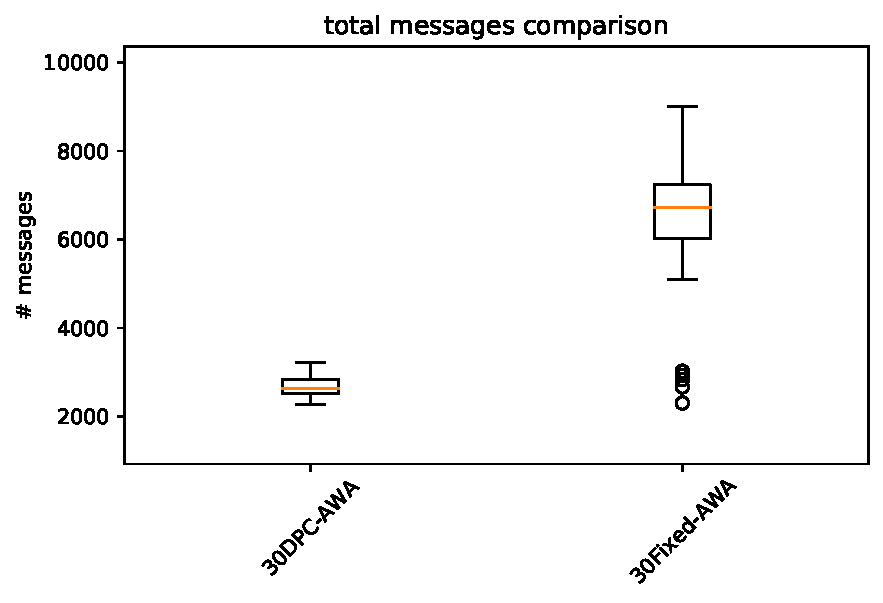
\includegraphics[width=\textwidth]{images/internet_like/1000/comparison/comparison_AWA_messages_boxplot.pdf}
		 \caption{Network perforcances, messages necessary to reach convergence
			with different \ac{MRAI} strategies}
         \label{fig:boxplot_internet_like_1000_messages_AWA}
     \end{subfigure}
     \hfill
     \begin{subfigure}[b]{0.45\textwidth}
         \centering
         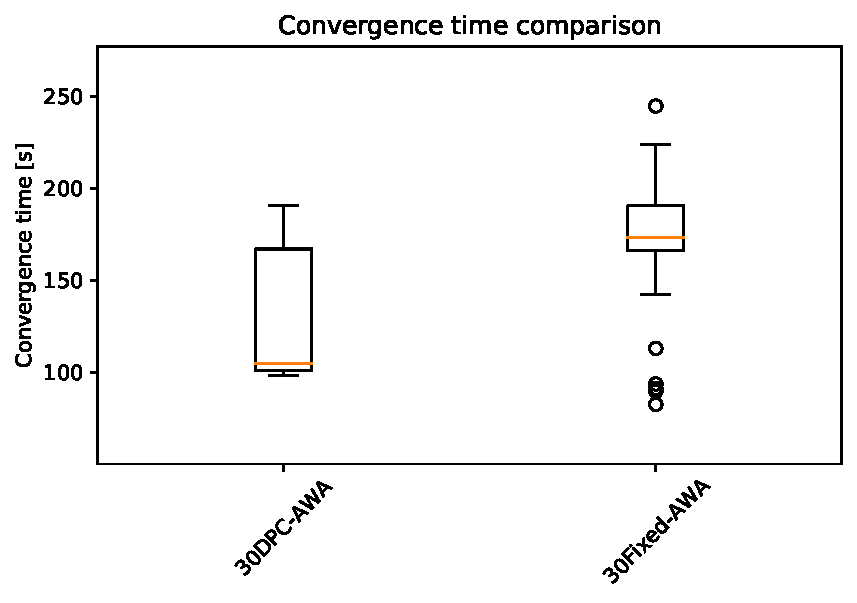
\includegraphics[width=\textwidth]{images/internet_like/1000/comparison/comparison_AWA_time_boxplot.pdf}
		 \caption{Network perforcances, time required to reach convergence
			with different \ac{MRAI} strategies}
         \label{fig:boxplot_internet_like_1000_time_AWA}
     \end{subfigure}
	 \caption{Network perfomances comparison with different \ac{MRAI} strategies,
		Graph internet like with \num{1000} nodes, \ac{MRAI} value
		\SI{30}{\second}, number of runs for each strategy \num{100}, signal \q{AWA}}
        \label{fig:boxplot_internet_like_1000_AWA}
\end{figure}

\begin{figure}[h]
     \centering
     \begin{subfigure}[b]{0.45\textwidth}
         \centering
         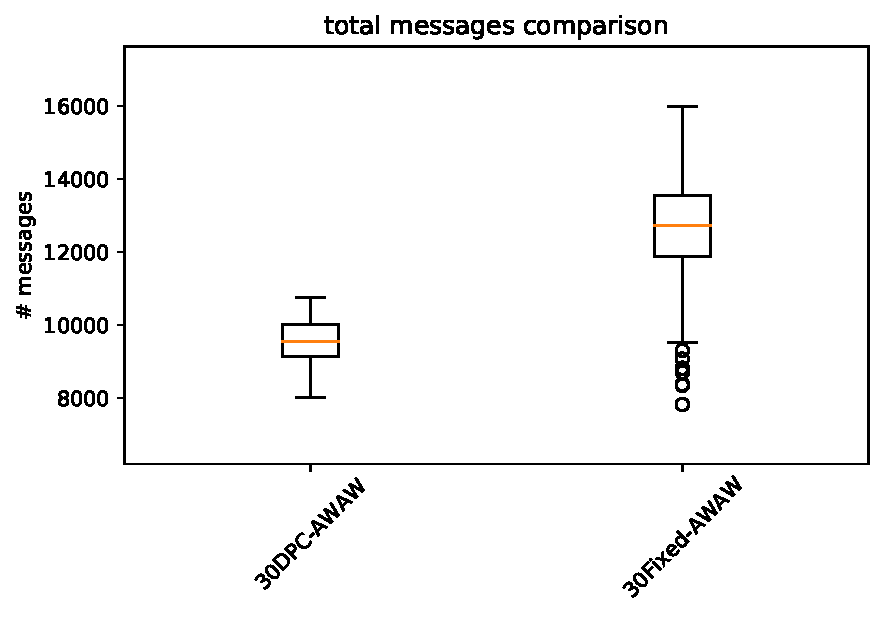
\includegraphics[width=\textwidth]{images/internet_like/1000/comparison/comparison_AWAW_messages_boxplot.pdf}
		 \caption{Network perforcances, messages necessary to reach convergence
			with different \ac{MRAI} strategies}
         \label{fig:boxplot_internet_like_1000_messages_AWAW}
     \end{subfigure}
     \hfill
     \begin{subfigure}[b]{0.45\textwidth}
         \centering
         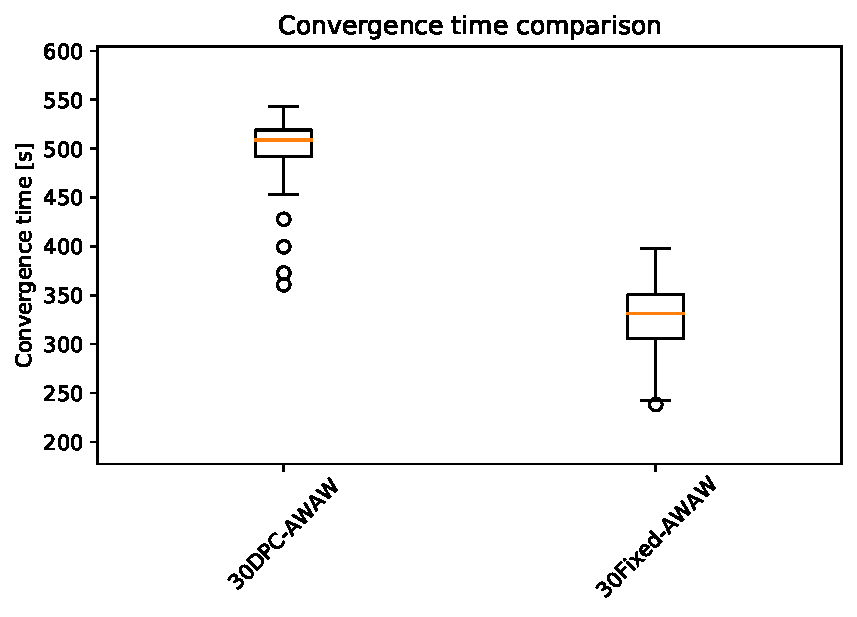
\includegraphics[width=\textwidth]{images/internet_like/1000/comparison/comparison_AWAW_time_boxplot.pdf}
		 \caption{Network perforcances, time required to reach convergence
			with different \ac{MRAI} strategies}
         \label{fig:boxplot_internet_like_1000_time_AWAW}
     \end{subfigure}
	 \caption{Network perfomances comparison with different \ac{MRAI} strategies,
		Graph internet like with \num{1000} nodes, \ac{MRAI} value
		\SI{30}{\second}, number of runs for each strategy \num{100}, signal \q{AWAW}}
        \label{fig:boxplot_internet_like_1000_AWAW}
\end{figure}

\begin{figure}[h]
     \centering
     \begin{subfigure}[b]{0.45\textwidth}
         \centering
         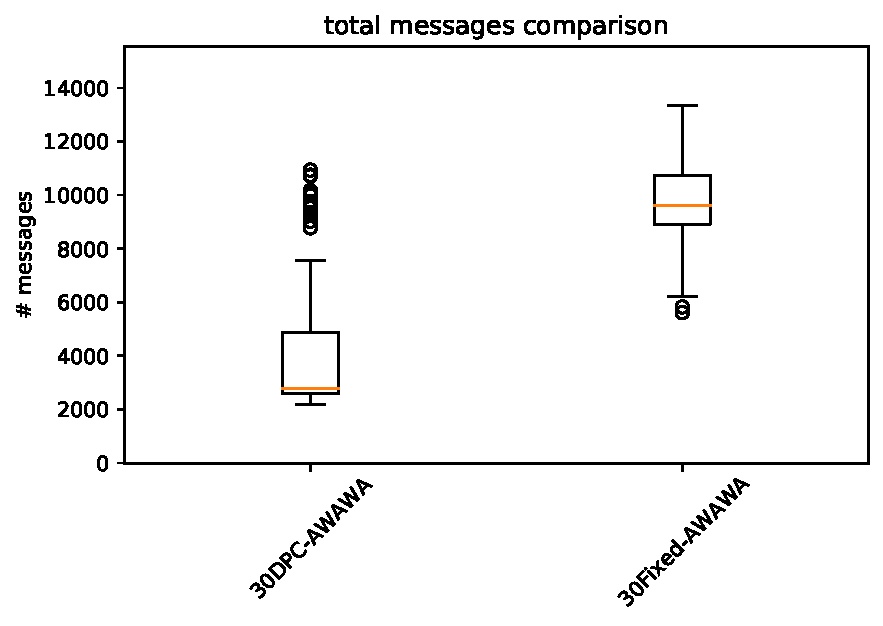
\includegraphics[width=\textwidth]{images/internet_like/1000/comparison/comparison_AWAWA_messages_boxplot.pdf}
		 \caption{Network perforcances, messages necessary to reach convergence
			with different \ac{MRAI} strategies}
         \label{fig:boxplot_internet_like_1000_messages_AWAWA}
     \end{subfigure}
     \hfill
     \begin{subfigure}[b]{0.45\textwidth}
         \centering
         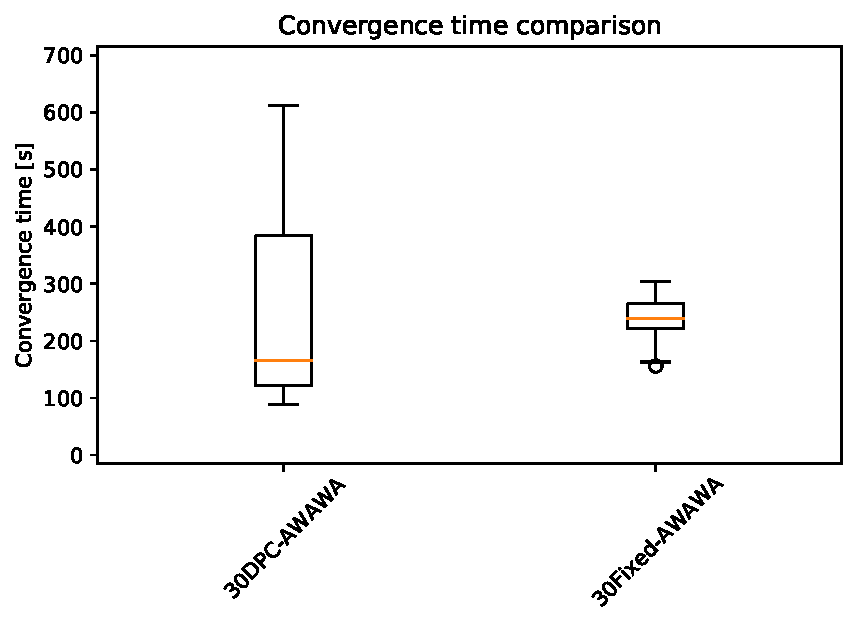
\includegraphics[width=\textwidth]{images/internet_like/1000/comparison/comparison_AWAWA_time_boxplot.pdf}
		 \caption{Network perforcances, time required to reach convergence
			with different \ac{MRAI} strategies}
         \label{fig:boxplot_internet_like_1000_time_AWAWA}
     \end{subfigure}
	 \caption{Network perfomances comparison with different \ac{MRAI} strategies,
		Graph internet like with \num{1000} nodes, \ac{MRAI} value
		\SI{30}{\second}, number of runs for each strategy \num{100}, signal \q{AWAWA}}
        \label{fig:boxplot_internet_like_1000_AWAWA}
\end{figure}

\begin{figure}[h]
    \centering
    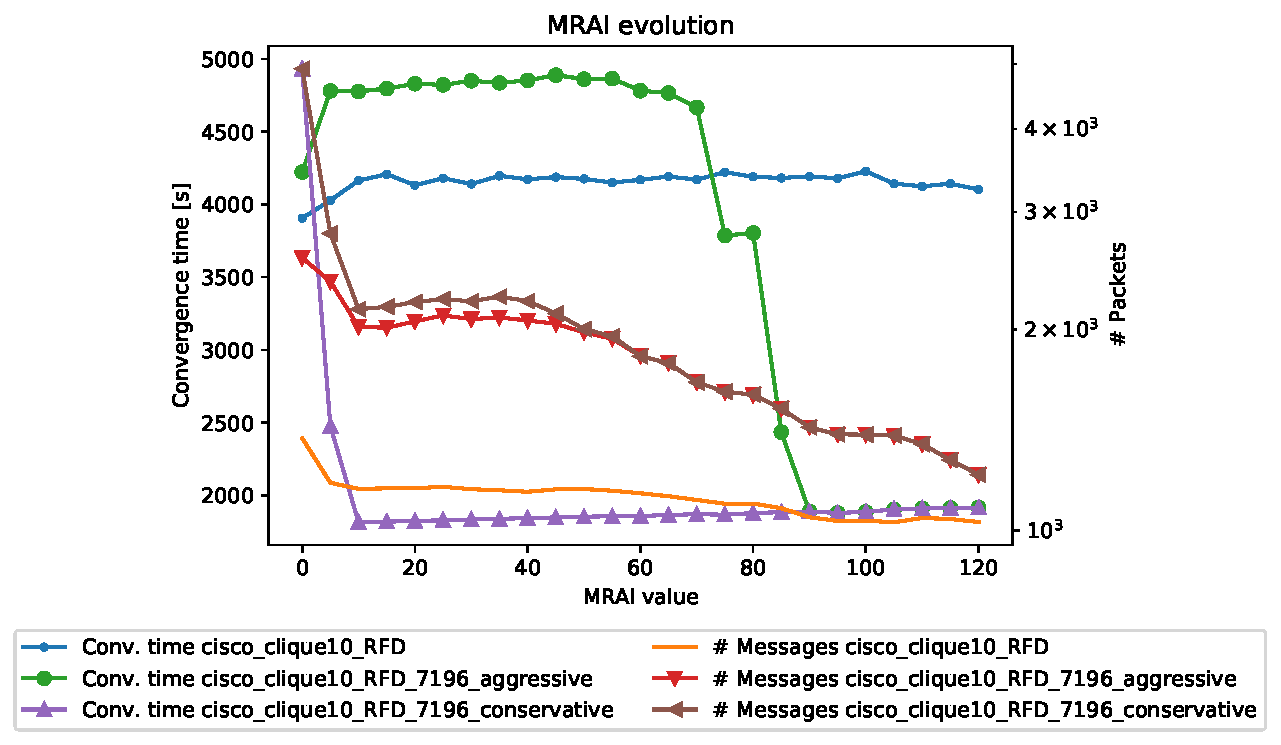
\includegraphics[width=\textwidth]{images/RFD/clique/cisco_clique10_RFD_comparison_constant_all.pdf}
	\caption{Comparison of the \textit{clique} topology with RFD 2439 and the with
		RFD 7196 strategies}
    \label{fig:clique_RFD2439VSRFD7196}
\end{figure}

%\begin{figure}[h]
%     \centering
%     \begin{subfigure}[b]{0.3\textwidth}
%         \centering
%         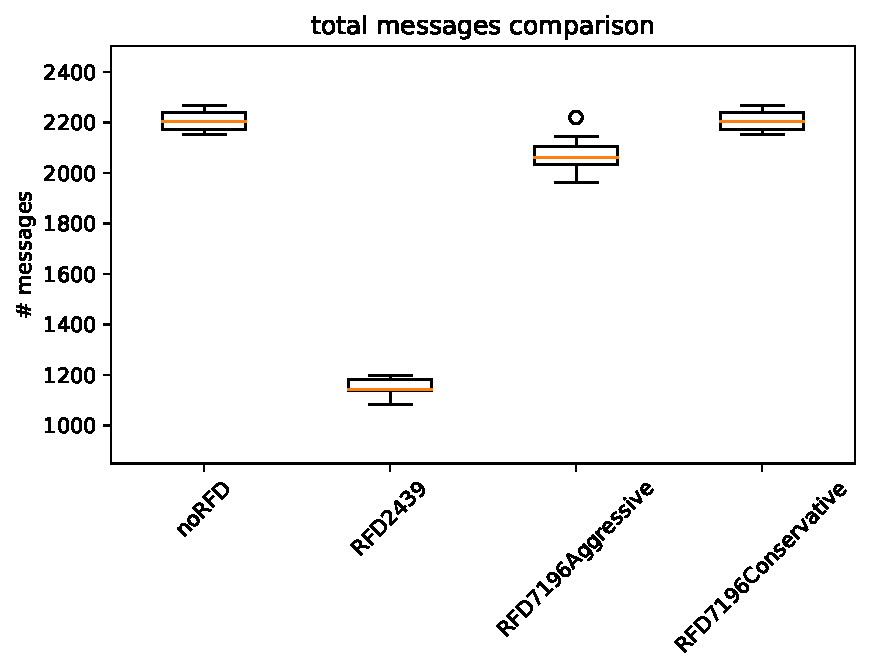
\includegraphics[width=\textwidth]{images/RFD/clique/clique_rfd_comparison_messages_boxplot.pdf}
%         \caption{clique topology, MRAI=30s, 10 runs, Messages comparison}
%         \label{fig:RFD_MRAI30_messages}
%     \end{subfigure}
%     \hfill
%     \begin{subfigure}[b]{0.3\textwidth}
%         \centering
%         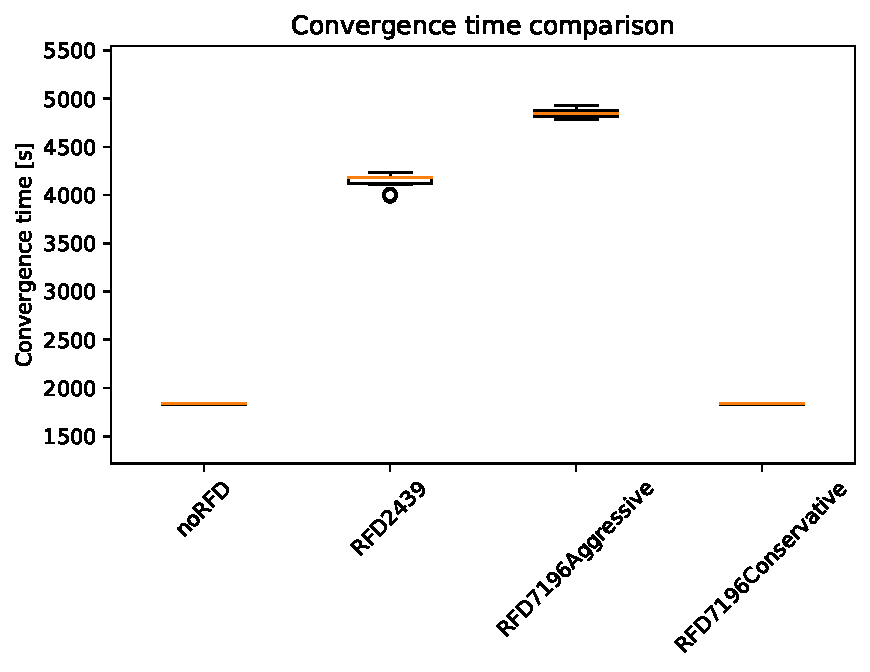
\includegraphics[width=\textwidth]{images/RFD/clique/clique_rfd_comparison_time_boxplot.pdf}
%         \caption{clique topology, MRAI=30s, 10 runs, Convergence time}
%         \label{fig:RFD_MRAI30_convTime}
%     \end{subfigure}
%     \hfill
%     \begin{subfigure}[b]{0.3\textwidth}
%         \centering
%         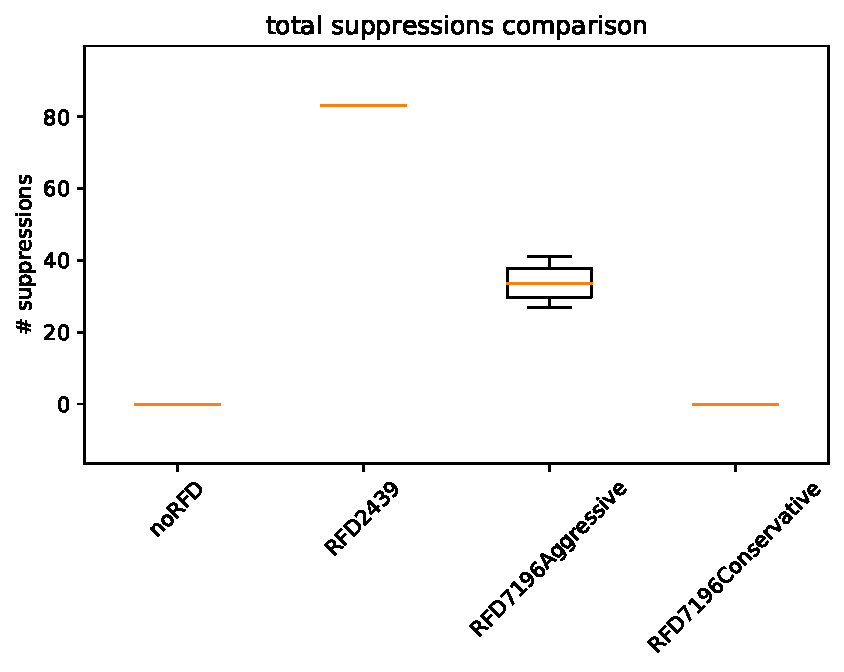
\includegraphics[width=\textwidth]{images/RFD/clique/clique_rfd_comparison_suppressions_boxplot.pdf}
%         \caption{clique topology, MRAI=30s, 10 runs, Number of suppressions}
%         \label{fig:RFD_MRAI30_suppressions}
%     \end{subfigure}
%        \caption{Clique topology, MRAI=30s, 10 runs, comparison of the network performances}
%        \label{fig:RFD_MRAI30}
%\end{figure}
\clearpage

\begin{figure}[H]
     \centering
     \begin{subfigure}[b]{0.325\textwidth}
         \centering
         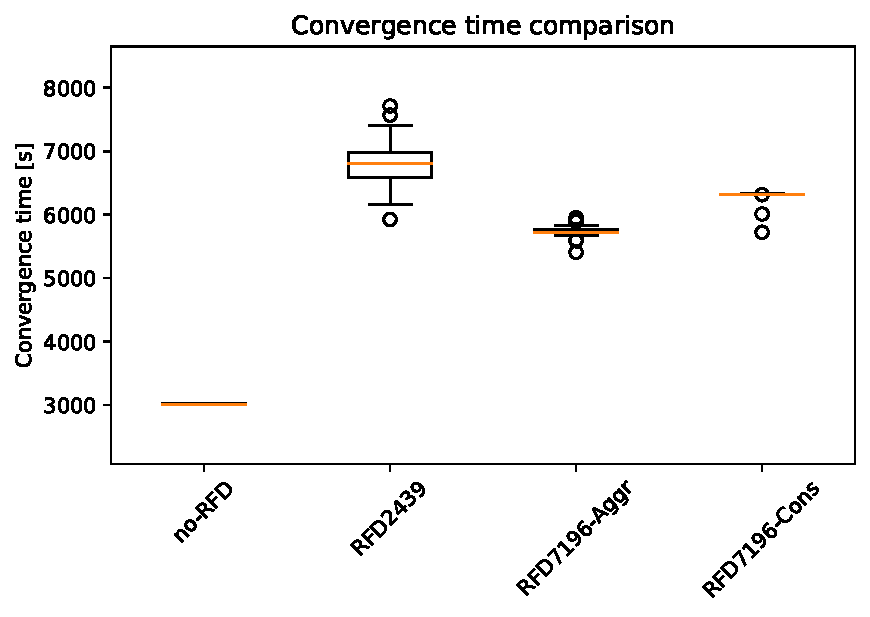
\includegraphics[width=\textwidth]{images/RFD/miceVSelephants/MultiMRAI/0/mice/cisco_1000MRAI0_rfd_comparison_time_boxplot.pdf}
         \caption{Convergence time respect to the RFD strategy, MRAI=0s}
         \label{fig:1000_RFD_MRAI0_time_mice}
     \end{subfigure}
     \hfill
     \begin{subfigure}[b]{0.325\textwidth}
         \centering
         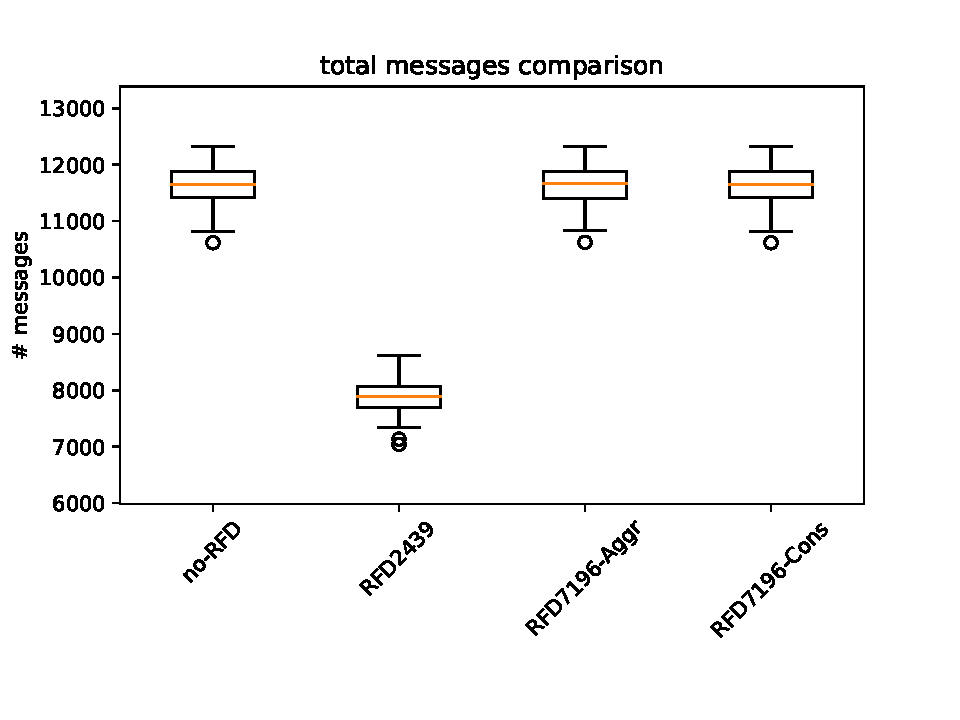
\includegraphics[width=\textwidth]{images/RFD/miceVSelephants/MultiMRAI/0/mice/cisco_1000MRAI0_rfd_comparison_messages_boxplot.pdf}
         \caption{Number of messages respect to the RFD strategy, MRAI=0s}
         \label{fig:1000_RFD_MRAI0_messages_mice}
     \end{subfigure}
     \hfill
     \begin{subfigure}[b]{0.325\textwidth}
         \centering
         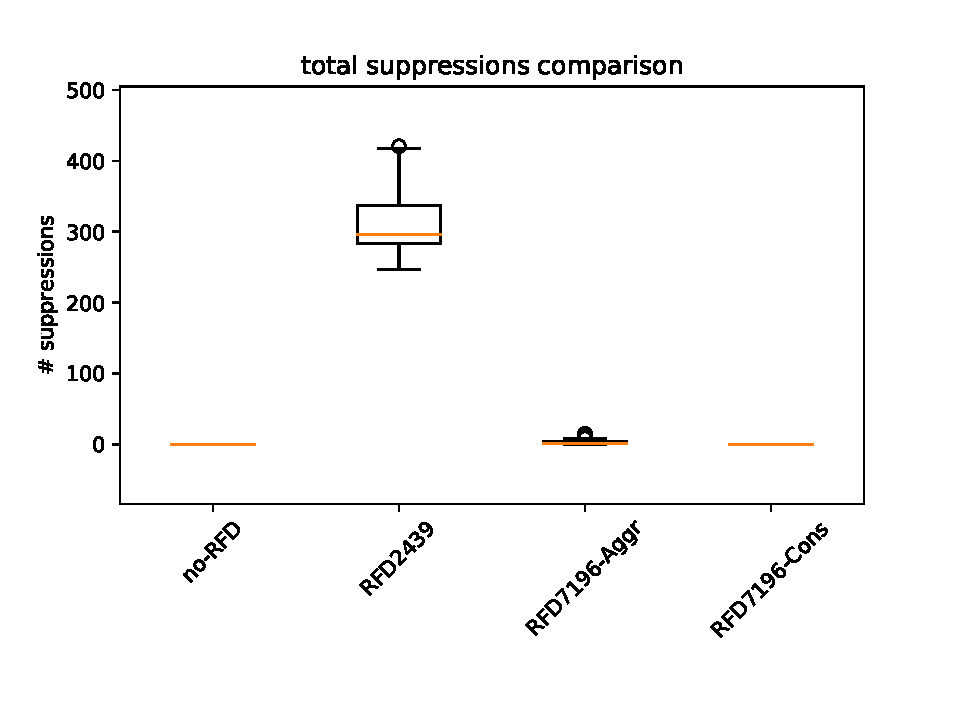
\includegraphics[width=\textwidth]{images/RFD/miceVSelephants/MultiMRAI/0/mice/cisco_1000MRAI0_rfd_comparison_suppressions_boxplot.pdf}
         \caption{Number of suppressions respect to the RFD strategy, MRAI=0s}
         \label{fig:1000_RFD_MRAI0_suppressions_mice}
     \end{subfigure}
     \vfill
     \begin{subfigure}[b]{0.325\textwidth}
         \centering
         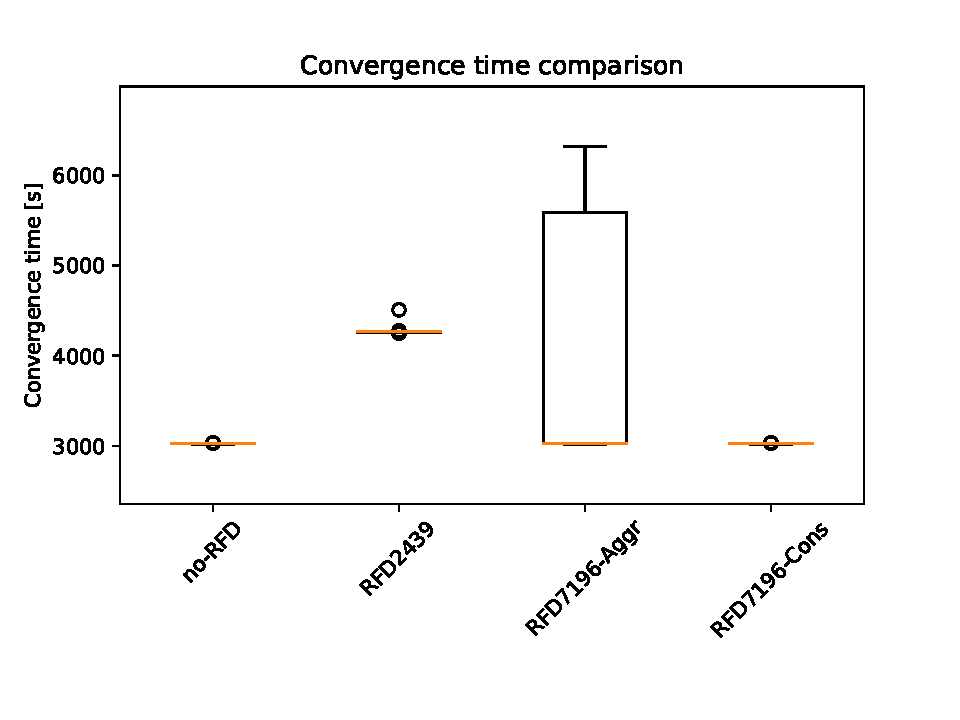
\includegraphics[width=\textwidth]{images/RFD/miceVSelephants/MultiMRAI/15/mice/cisco_1000MRAI15_rfd_comparison_time_boxplot.pdf}
         \caption{Convergence time respect to the RFD strategy, MRAI=15s}
         \label{fig:1000_RFD_MRAI15_time_mice}
     \end{subfigure}
     \hfill
     \begin{subfigure}[b]{0.325\textwidth}
         \centering
         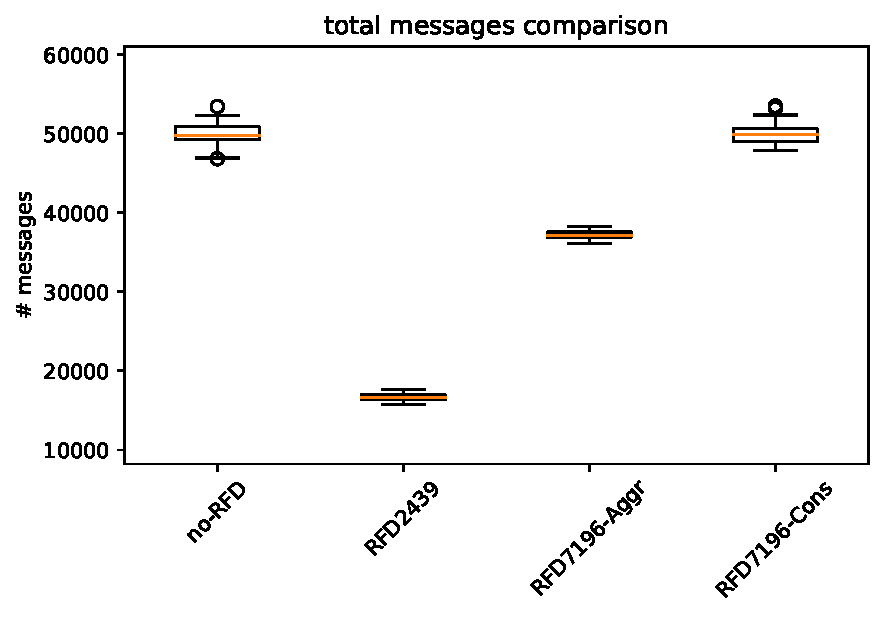
\includegraphics[width=\textwidth]{images/RFD/miceVSelephants/MultiMRAI/15/mice/cisco_1000MRAI15_rfd_comparison_messages_boxplot.pdf}
         \caption{Number of messages respect to the RFD strategy, MRAI=15s}
         \label{fig:1000_RFD_MRAI15_messages_mice}
     \end{subfigure}
     \hfill
     \begin{subfigure}[b]{0.325\textwidth}
         \centering
         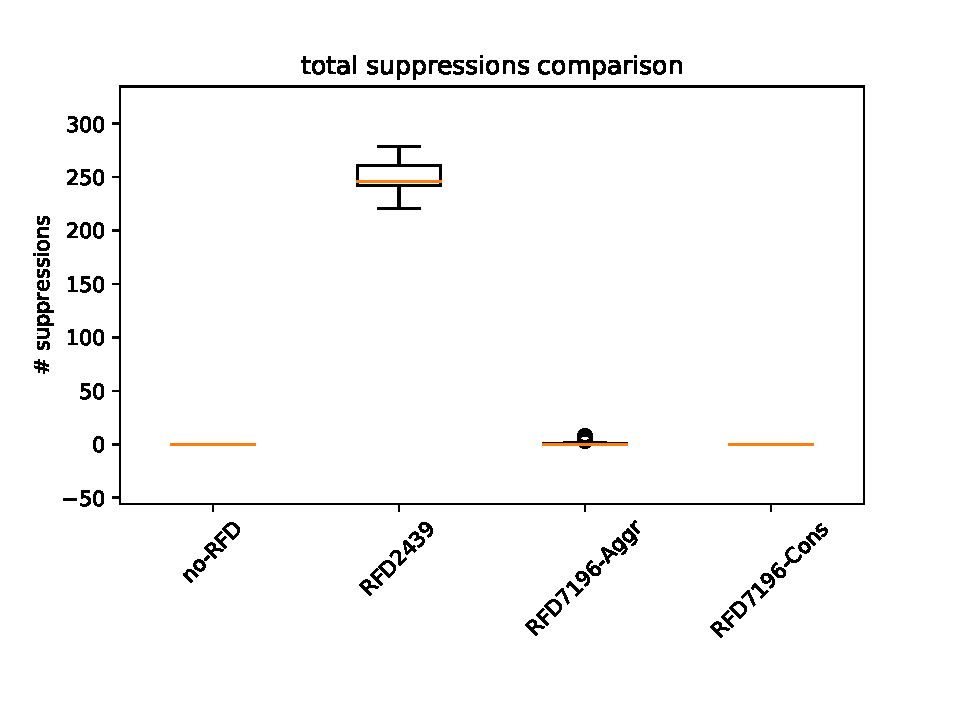
\includegraphics[width=\textwidth]{images/RFD/miceVSelephants/MultiMRAI/15/mice/cisco_1000MRAI15_rfd_comparison_suppressions_boxplot.pdf}
         \caption{Number of suppressions respect to the RFD strategy, MRAI=15s}
         \label{fig:1000_RFD_MRAI15_suppressions_mice}
     \end{subfigure}
     \vfill
     \begin{subfigure}[b]{0.325\textwidth}
         \centering
         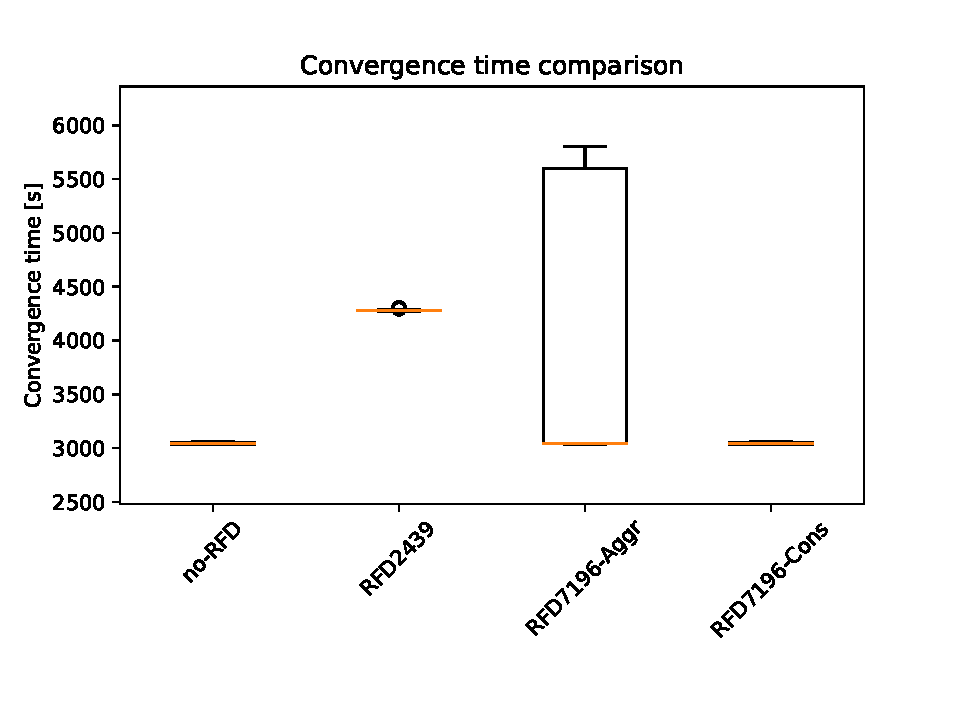
\includegraphics[width=\textwidth]{images/RFD/miceVSelephants/MultiMRAI/30/mice/cisco_1000MRAI30_rfd_comparison_time_boxplot.pdf}
         \caption{Convergence time respect to the RFD strategy, MRAI=30s}
         \label{fig:1000_RFD_MRAI30_time_mice}
     \end{subfigure}
     \hfill
     \begin{subfigure}[b]{0.325\textwidth}
         \centering
         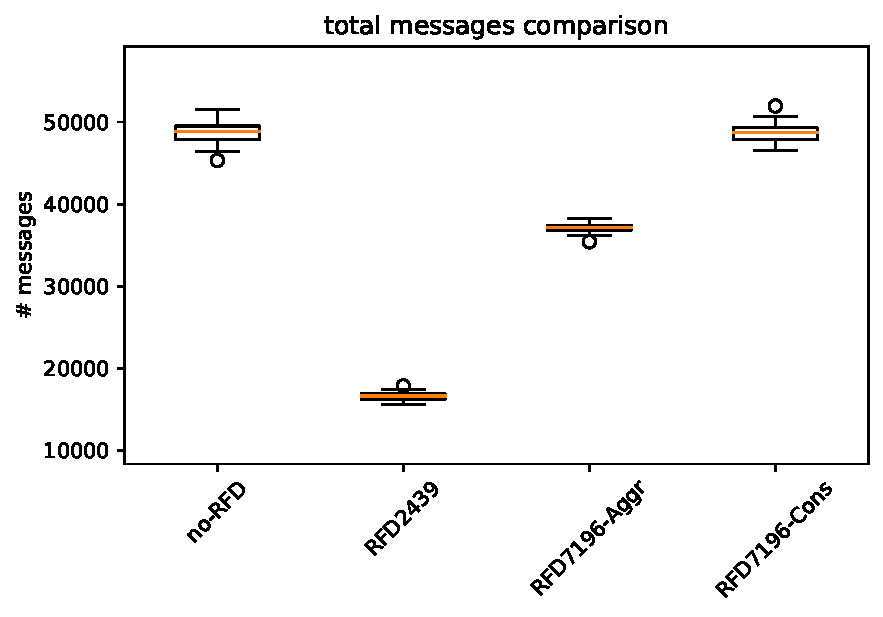
\includegraphics[width=\textwidth]{images/RFD/miceVSelephants/MultiMRAI/30/mice/cisco_1000MRAI30_rfd_comparison_messages_boxplot.pdf}
         \caption{Number of messages respect to the RFD strategy, MRAI=30s}
         \label{fig:1000_RFD_MRAI30_messages_mice}
     \end{subfigure}
     \hfill
     \begin{subfigure}[b]{0.325\textwidth}
         \centering
         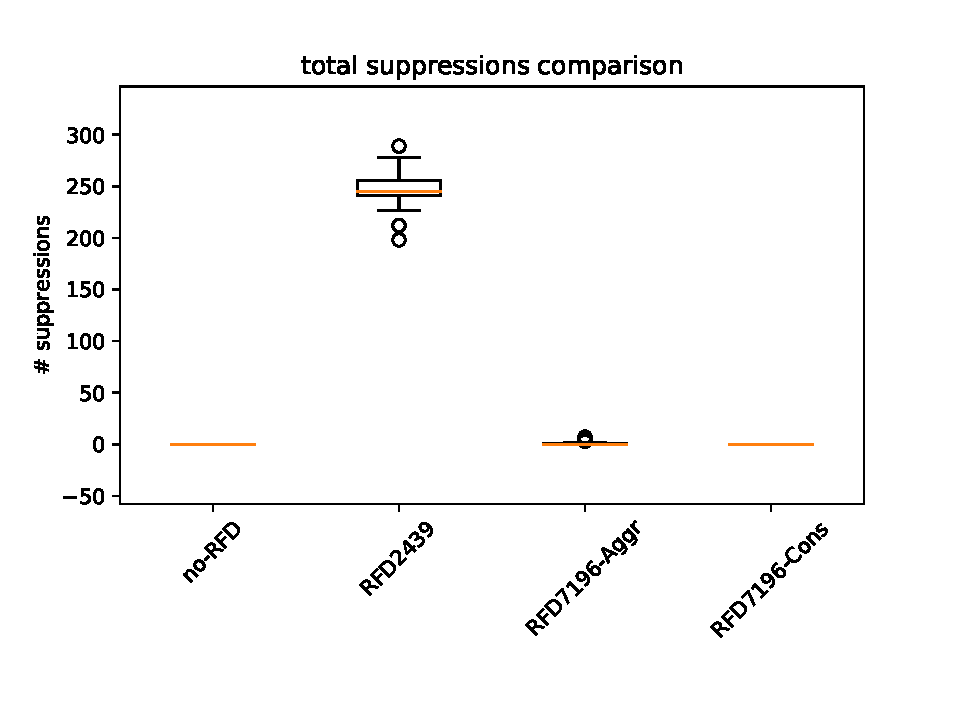
\includegraphics[width=\textwidth]{images/RFD/miceVSelephants/MultiMRAI/30/mice/cisco_1000MRAI30_rfd_comparison_suppressions_boxplot.pdf}
         \caption{Number of suppressions respect to the RFD strategy, MRAI=30s}
         \label{fig:1000_RFD_MRAI30_suppressions_mice}
     \end{subfigure}
     \vfill
     \begin{subfigure}[b]{0.325\textwidth}
         \centering
         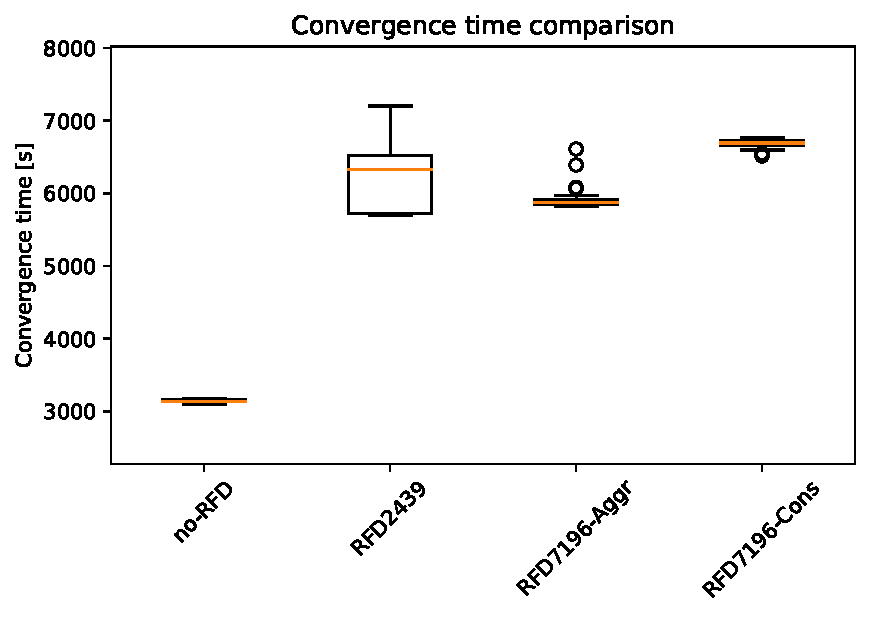
\includegraphics[width=\textwidth]{images/RFD/miceVSelephants/MultiMRAI/45/mice/cisco_1000MRAI45_rfd_comparison_time_boxplot.pdf}
         \caption{Convergence time respect to the RFD strategy, MRAI=45s}
         \label{fig:1000_RFD_MRAI45_time_mice}
     \end{subfigure}
     \hfill
     \begin{subfigure}[b]{0.325\textwidth}
         \centering
         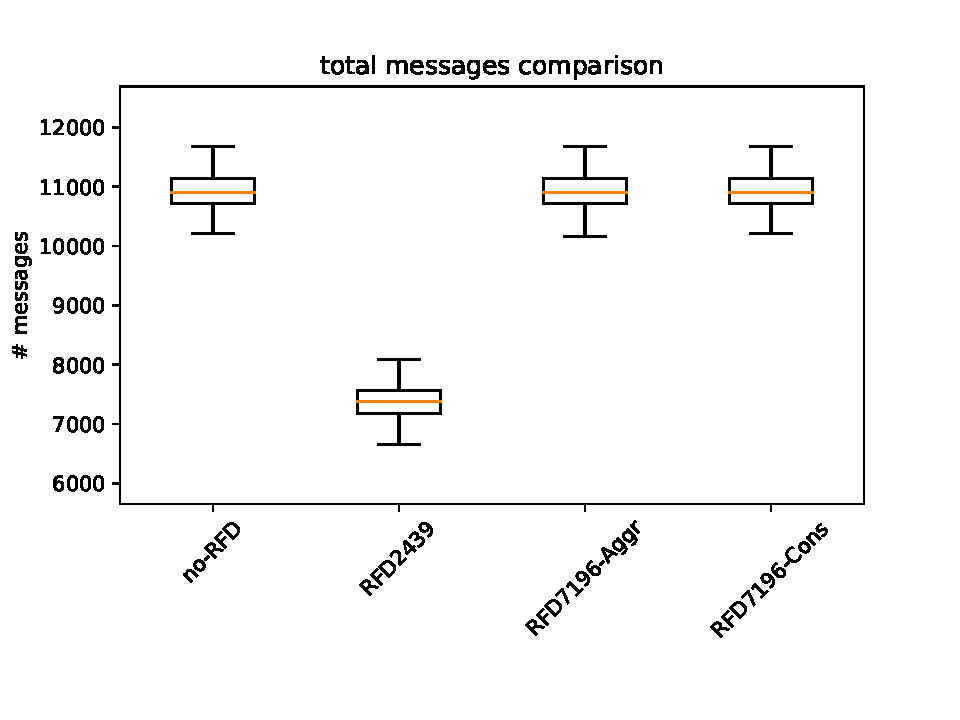
\includegraphics[width=\textwidth]{images/RFD/miceVSelephants/MultiMRAI/45/mice/cisco_1000MRAI45_rfd_comparison_messages_boxplot.pdf}
         \caption{Number of messages respect to the RFD strategy, MRAI=30s}
         \label{fig:1000_RFD_MRAI45_messages_mice}
     \end{subfigure}
     \hfill
     \begin{subfigure}[b]{0.325\textwidth}
         \centering
         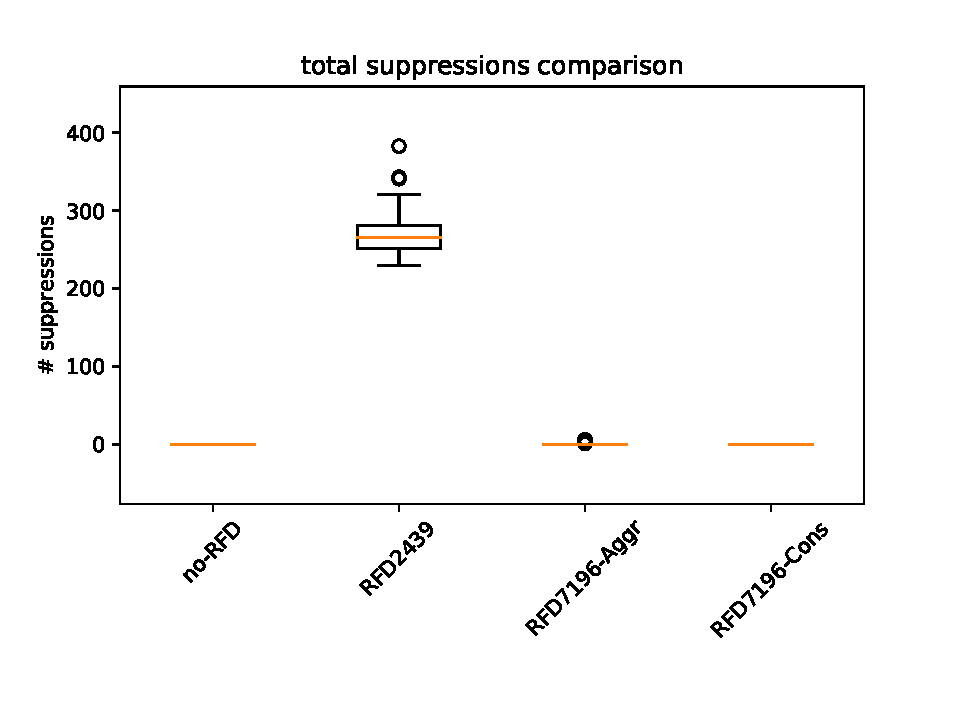
\includegraphics[width=\textwidth]{images/RFD/miceVSelephants/MultiMRAI/45/mice/cisco_1000MRAI45_rfd_comparison_suppressions_boxplot.pdf}
         \caption{Number of suppressions respect to the RFD strategy, MRAI=45s}
         \label{fig:1000_RFD_MRAI45_suppressions_mice}
     \end{subfigure}
     \vfill
     \begin{subfigure}[b]{0.325\textwidth}
         \centering
         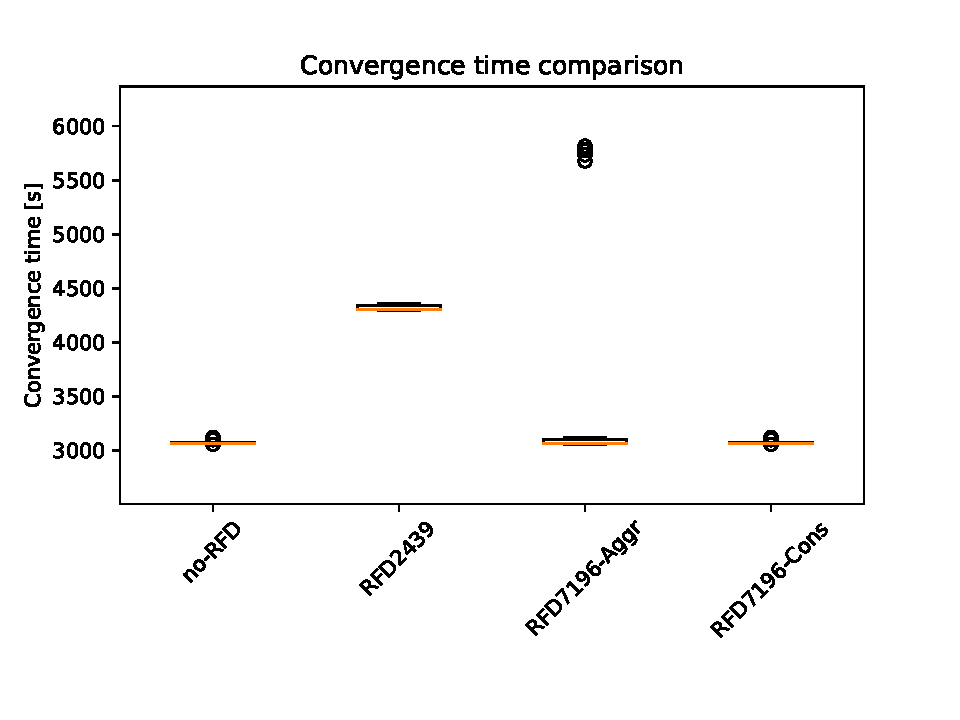
\includegraphics[width=\textwidth]{images/RFD/miceVSelephants/MultiMRAI/60/mice/cisco_1000MRAI60_rfd_comparison_time_boxplot.pdf}
         \caption{Convergence time respect to the RFD strategy, MRAI=60s}
         \label{fig:1000_RFD_MRAI60_time_mice}
     \end{subfigure}
     \hfill
     \begin{subfigure}[b]{0.325\textwidth}
         \centering
         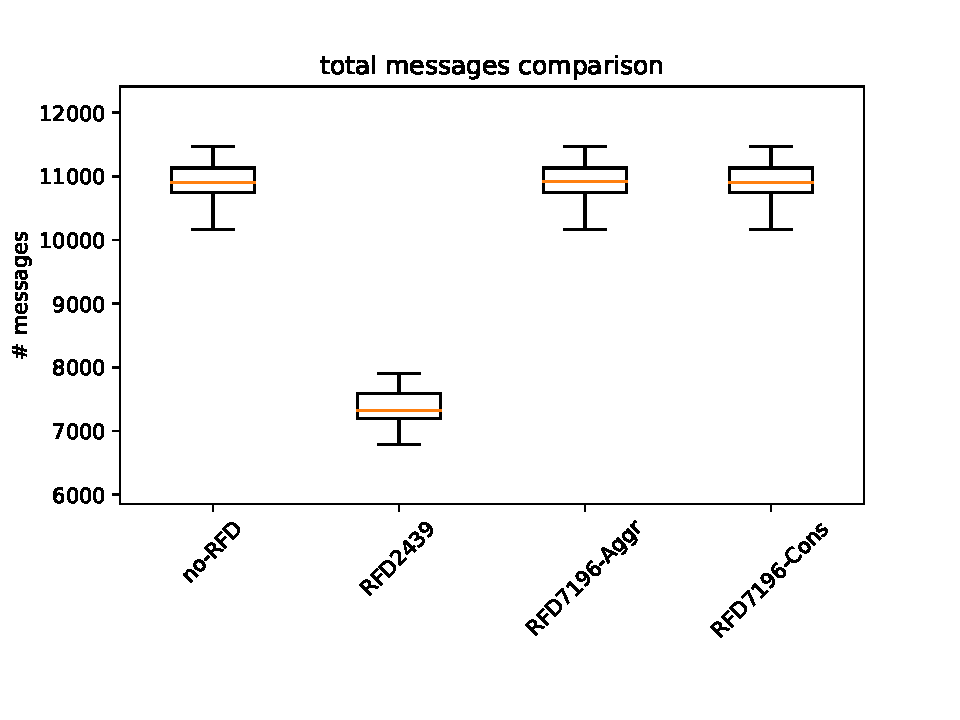
\includegraphics[width=\textwidth]{images/RFD/miceVSelephants/MultiMRAI/60/mice/cisco_1000MRAI60_rfd_comparison_messages_boxplot.pdf}
         \caption{Number of messages respect to the RFD strategy, MRAI=60s}
         \label{fig:1000_RFD_MRAI60_messages_mice}
     \end{subfigure}
     \hfill
     \begin{subfigure}[b]{0.325\textwidth}
         \centering
         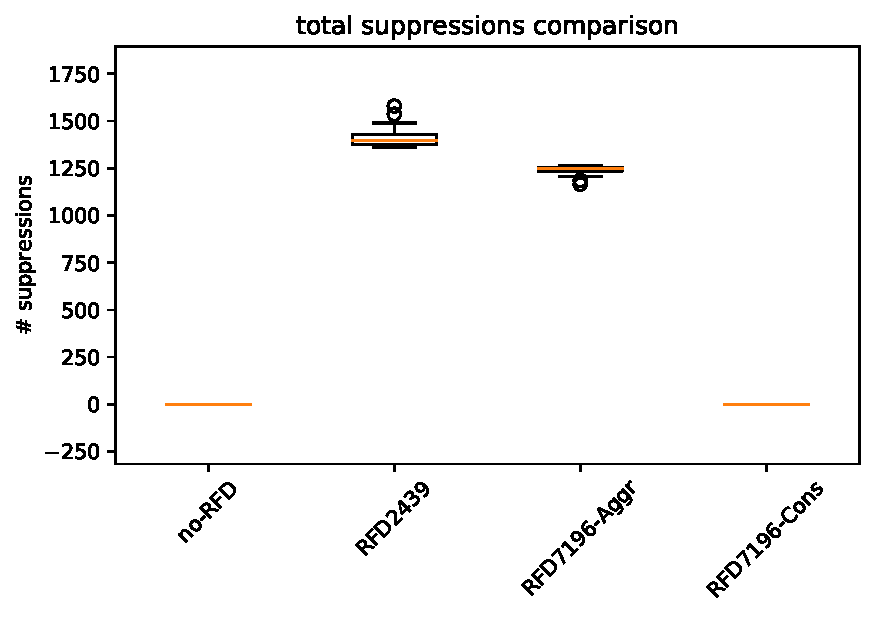
\includegraphics[width=\textwidth]{images/RFD/miceVSelephants/MultiMRAI/60/mice/cisco_1000MRAI60_rfd_comparison_suppressions_boxplot.pdf}
         \caption{Number of suppressions respect to the RFD strategy, MRAI=60s}
         \label{fig:1000_RFD_MRAI60_suppressions_mice}
     \end{subfigure}
        \caption{Internet like topology 1000 nodes, random destination, 5 flaps, 300s delay, Network performances}
        \label{fig:1000_RFD_MRAI30_mice}
\end{figure}

\begin{figure}[H]
     \centering
     \begin{subfigure}[b]{0.325\textwidth}
         \centering
         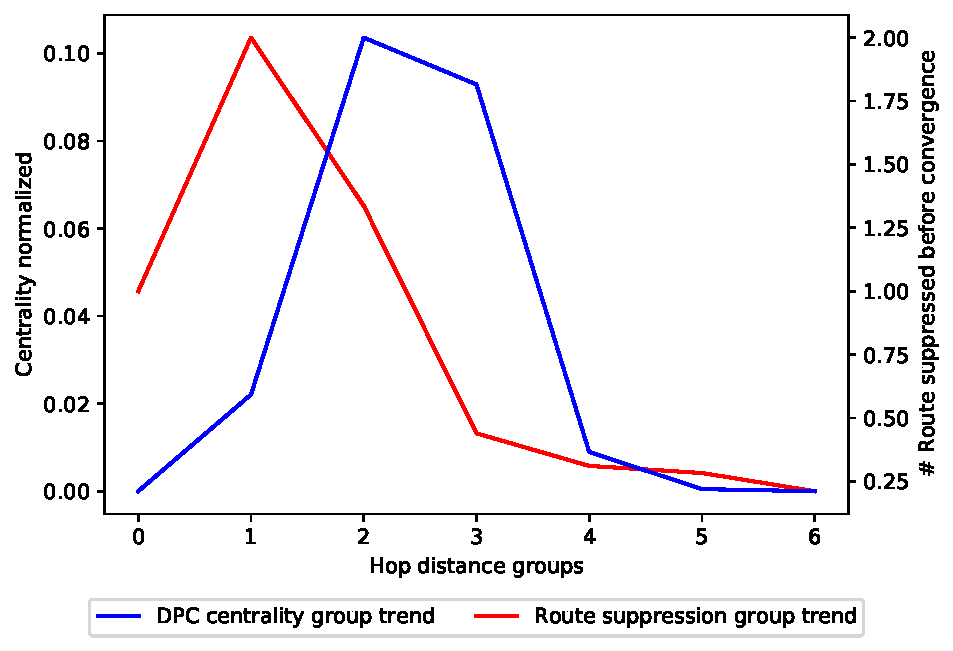
\includegraphics[width=\textwidth]{images/RFD/miceVSelephants/MultiMRAI/0/mice/cisco_1000_RFD_nodeConvergence_centVSsup_trend.pdf}
         \caption{RFD 2439 Strategy, \\MRAI=0s}
         \label{fig:1000_2439RFD_centVSsup_mices_MRAI0}
     \end{subfigure}
     \hfill
     \begin{subfigure}[b]{0.325\textwidth}
         \centering
         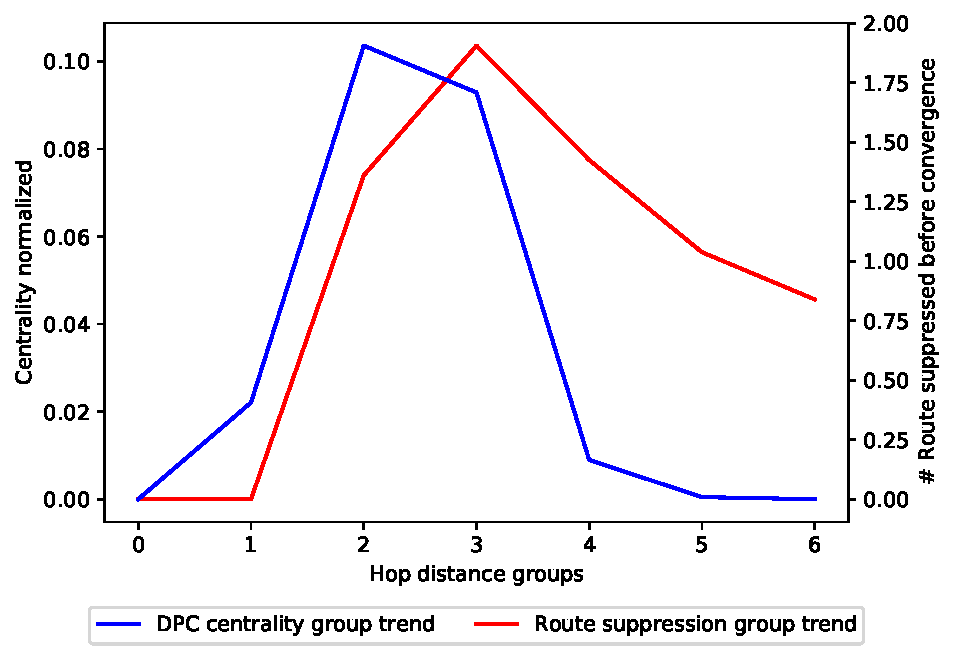
\includegraphics[width=\textwidth]{images/RFD/miceVSelephants/MultiMRAI/0/mice/cisco_1000_RFD_7196_aggressive_nodeConvergence_centVSsup_trend.pdf}
         \caption{RFD 7196 Aggressive Strategy, MRAI=0s}
         \label{fig:1000_7196RFDA_centVSsup_mices_MRAI0}
     \end{subfigure}
     \hfill
     \begin{subfigure}[b]{0.325\textwidth}
         \centering
         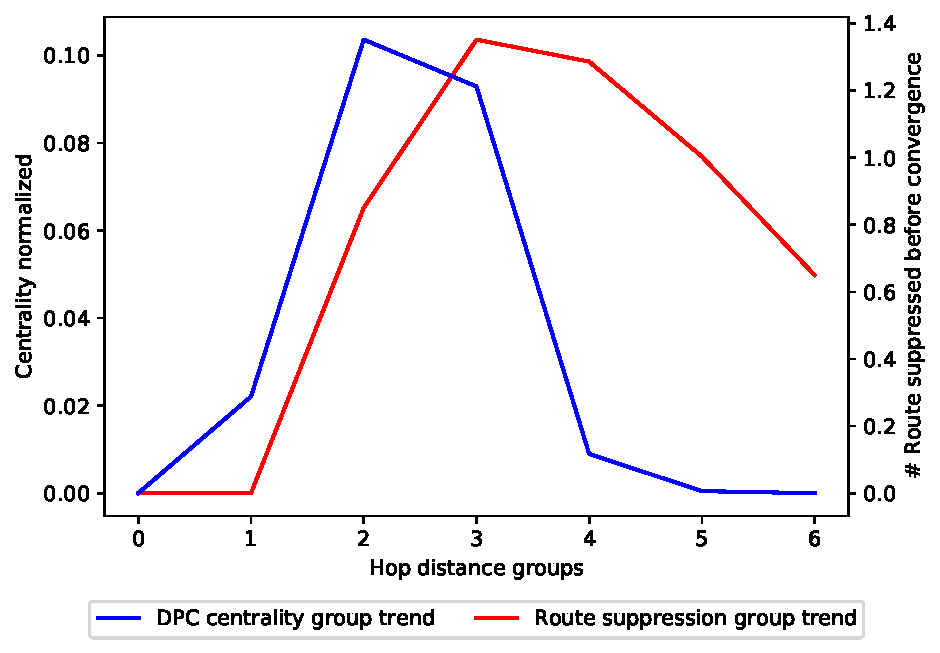
\includegraphics[width=\textwidth]{images/RFD/miceVSelephants/MultiMRAI/0/mice/cisco_1000_RFD_7196_conservative_nodeConvergence_centVSsup_trend.pdf}
         \caption{RFD 7196 Conservative Strategy, MRAI=0s}
         \label{fig:1000_7196RFDC_centVSsup_mices_MRAI0}
     \end{subfigure}
     \vfill
     \begin{subfigure}[b]{0.325\textwidth}
         \centering
         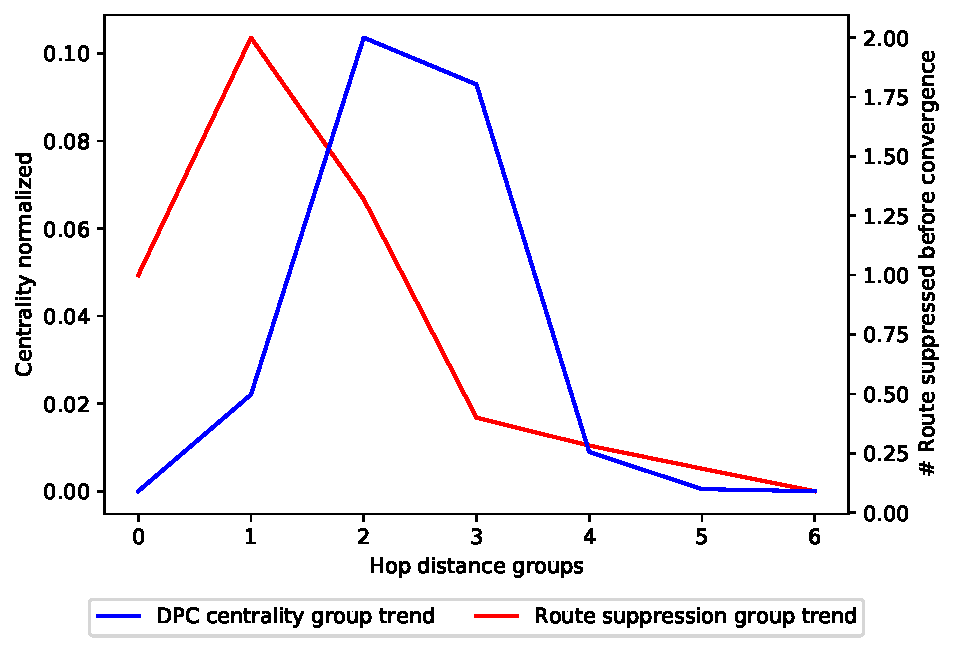
\includegraphics[width=\textwidth]{images/RFD/miceVSelephants/MultiMRAI/15/mice/cisco_1000_RFD_nodeConvergence_centVSsup_trend.pdf}
         \caption{RFD 2439 Strategy, \\MRAI=15s}
         \label{fig:1000_2439RFD_centVSsup_mices_MRAI15}
     \end{subfigure}
     \hfill
     \begin{subfigure}[b]{0.325\textwidth}
         \centering
         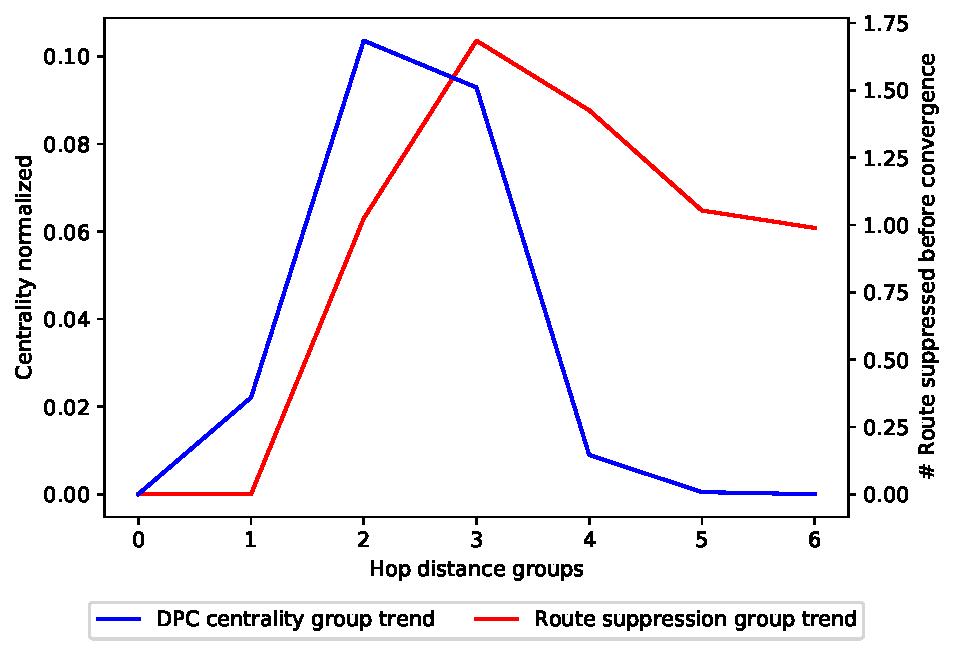
\includegraphics[width=\textwidth]{images/RFD/miceVSelephants/MultiMRAI/15/mice/cisco_1000_RFD_7196_aggressive_nodeConvergence_centVSsup_trend.pdf}
         \caption{RFD 7196 Aggressive Strategy, MRAI=15s}
         \label{fig:1000_7196RFDA_centVSsup_mices_MRAI15}
     \end{subfigure}
     \hfill
     \begin{subfigure}[b]{0.325\textwidth}
         \centering
         \includegraphics[width=\textwidth]{images/RFD/miceVSelephants/MultiMRAI/15/mice/cisco_1000_RFD_7196_conservative_nodeConvergence_centVSsup_trend.pdf}
         \caption{RFD 7196 Conservative Strategy, MRAI=15s}
         \label{fig:1000_7196RFDC_centVSsup_mices_MRAI15}
     \end{subfigure}
     \vfill
     \begin{subfigure}[b]{0.325\textwidth}
         \centering
         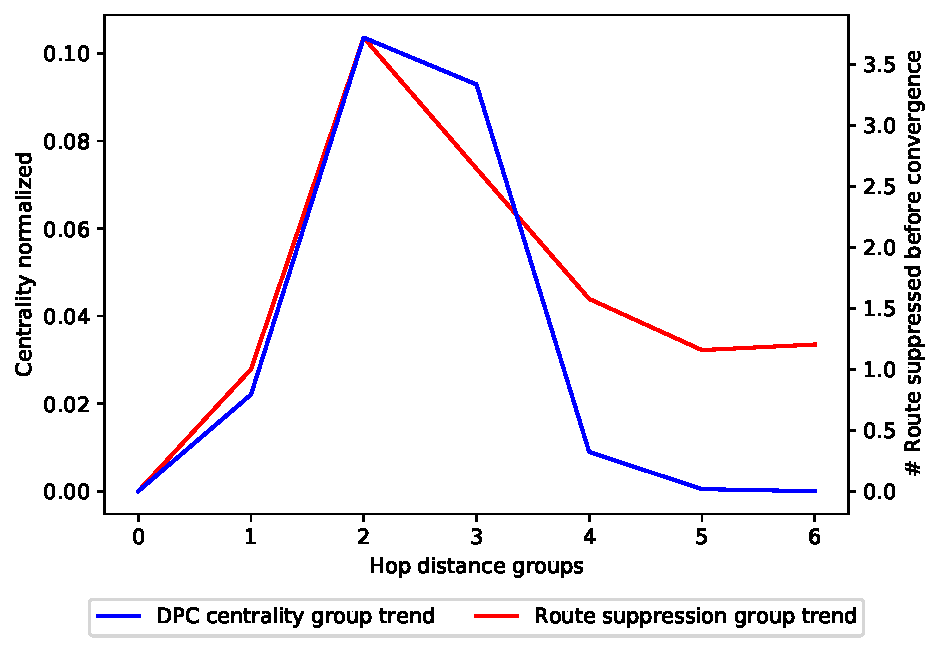
\includegraphics[width=\textwidth]{images/RFD/miceVSelephants/MultiMRAI/30/mice/cisco_1000_RFD_nodeConvergence_centVSsup_trend.pdf}
         \caption{RFD 2439 Strategy, \\MRAI=30s}
         \label{fig:1000_2439RFD_centVSsup_mices_MRAI30}
     \end{subfigure}
     \hfill
     \begin{subfigure}[b]{0.325\textwidth}
         \centering
         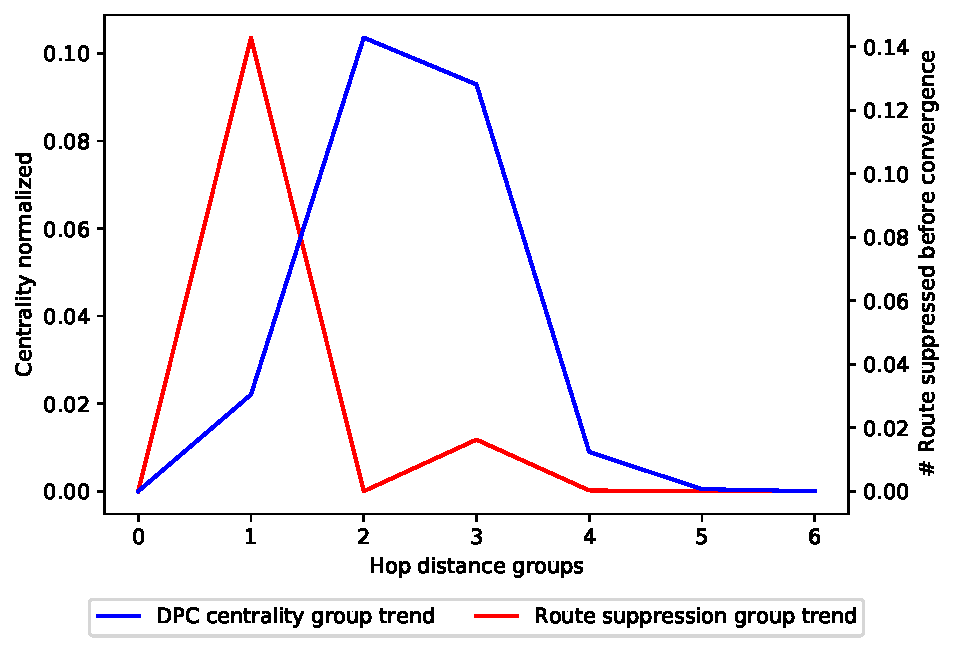
\includegraphics[width=\textwidth]{images/RFD/miceVSelephants/MultiMRAI/30/mice/cisco_1000_RFD_7196_aggressive_nodeConvergence_centVSsup_trend.pdf}
         \caption{RFD 7196 Aggressive Strategy, MRAI=30s}
         \label{fig:1000_7196RFDA_centVSsup_mices_MRAI30}
     \end{subfigure}
     \hfill
     \begin{subfigure}[b]{0.325\textwidth}
         \centering
         \includegraphics[width=\textwidth]{images/RFD/miceVSelephants/MultiMRAI/30/mice/cisco_1000_RFD_7196_conservative_nodeConvergence_centVSsup_trend.pdf}
         \caption{RFD 7196 Conservative Strategy, MRAI=30s}
         \label{fig:1000_7196RFDC_centVSsup_mices_MRAI30}
     \end{subfigure}
     \vfill
     \begin{subfigure}[b]{0.325\textwidth}
         \centering
         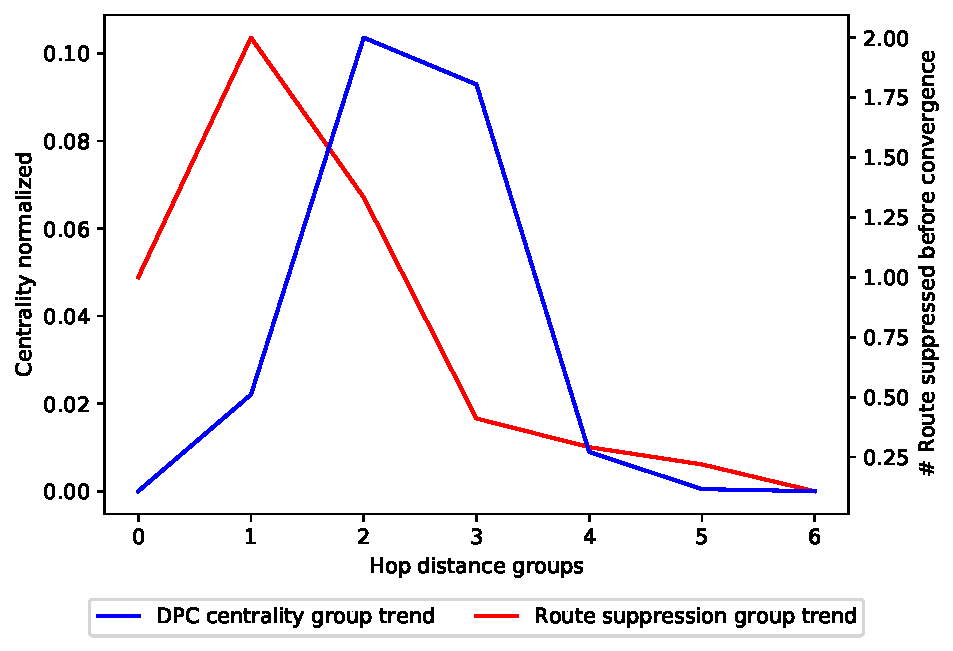
\includegraphics[width=\textwidth]{images/RFD/miceVSelephants/MultiMRAI/45/mice/cisco_1000_RFD_nodeConvergence_centVSsup_trend.pdf}
         \caption{RFD 2439 Strategy, \\MRAI=45s}
         \label{fig:1000_2439RFD_centVSsup_mices_MRAI45}
     \end{subfigure}
     \hfill
     \begin{subfigure}[b]{0.325\textwidth}
         \centering
         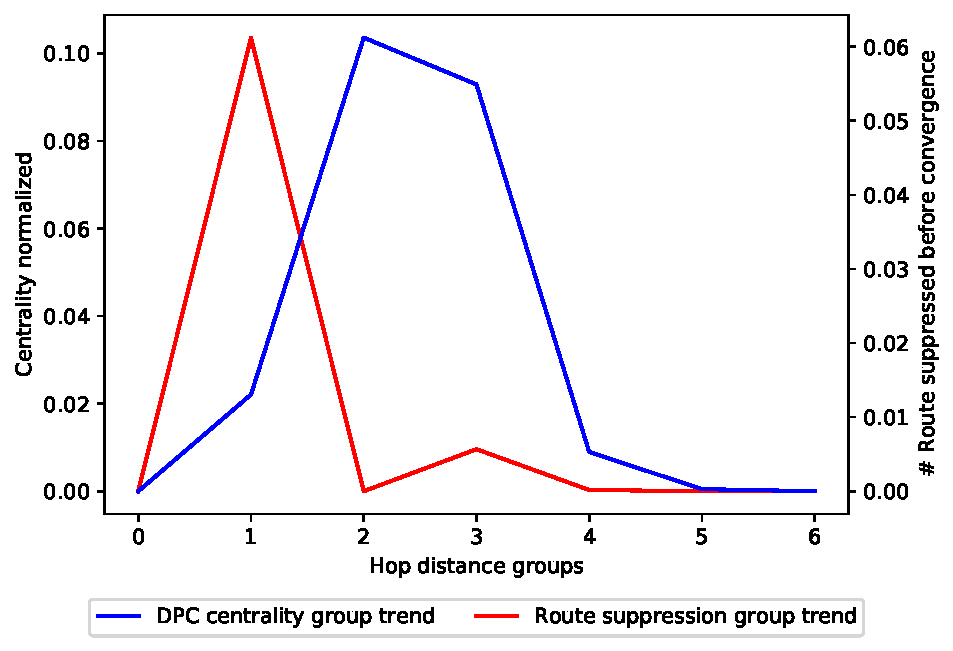
\includegraphics[width=\textwidth]{images/RFD/miceVSelephants/MultiMRAI/45/mice/cisco_1000_RFD_7196_aggressive_nodeConvergence_centVSsup_trend.pdf}
         \caption{RFD 7196 Aggressive Strategy, MRAI=45s}
         \label{fig:1000_7196RFDA_centVSsup_mices_MRAI45}
     \end{subfigure}
     \hfill
     \begin{subfigure}[b]{0.325\textwidth}
         \centering
         \includegraphics[width=\textwidth]{images/RFD/miceVSelephants/MultiMRAI/45/mice/cisco_1000_RFD_7196_conservative_nodeConvergence_centVSsup_trend.pdf}
         \caption{RFD 7196 Conservative Strategy, MRAI=45s}
         \label{fig:1000_7196RFDC_centVSsup_mices_MRAI45}
     \end{subfigure}
     \vfill
     \begin{subfigure}[b]{0.325\textwidth}
         \centering
         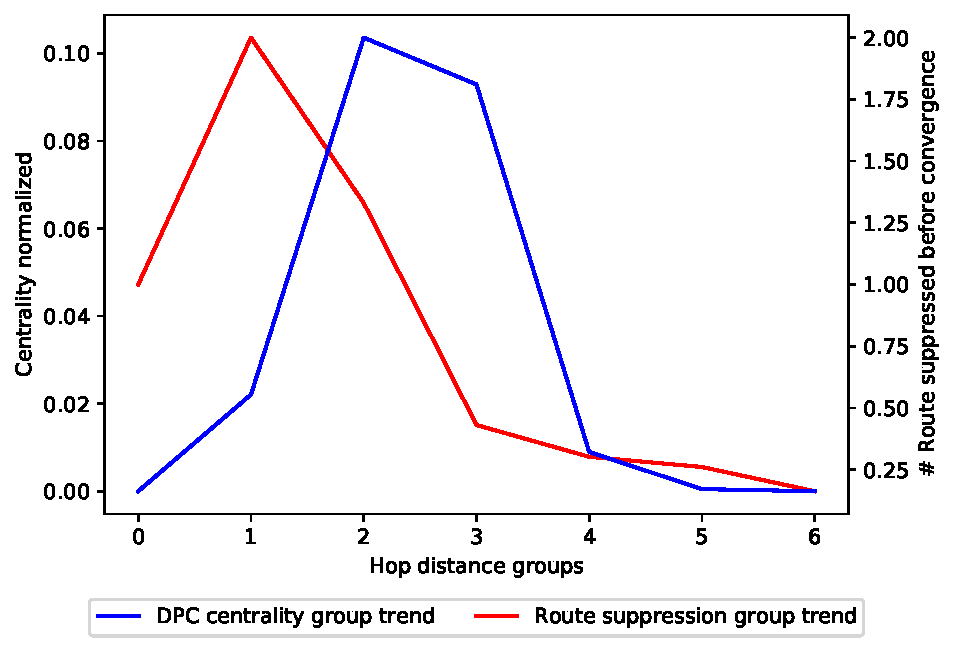
\includegraphics[width=\textwidth]{images/RFD/miceVSelephants/MultiMRAI/60/mice/cisco_1000_RFD_nodeConvergence_centVSsup_trend.pdf}
         \caption{RFD 2439 Strategy, \\MRAI=60s}
         \label{fig:1000_2439RFD_centVSsup_mices_MRAI60}
     \end{subfigure}
     \hfill
     \begin{subfigure}[b]{0.325\textwidth}
         \centering
         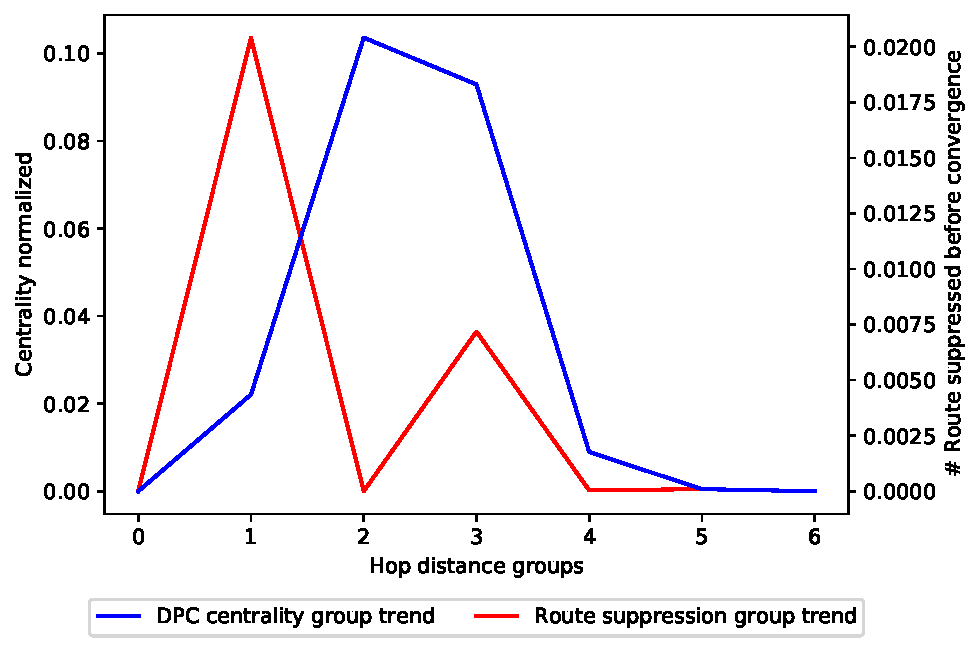
\includegraphics[width=\textwidth]{images/RFD/miceVSelephants/MultiMRAI/60/mice/cisco_1000_RFD_7196_aggressive_nodeConvergence_centVSsup_trend.pdf}
         \caption{RFD 7196 Aggressive Strategy, MRAI=60s}
         \label{fig:1000_7196RFDA_centVSsup_mices_MRAI60}
     \end{subfigure}
     \hfill
     \begin{subfigure}[b]{0.325\textwidth}
         \centering
         \includegraphics[width=\textwidth]{images/RFD/miceVSelephants/MultiMRAI/60/mice/cisco_1000_RFD_7196_conservative_nodeConvergence_centVSsup_trend.pdf}
         \caption{RFD 7196 Conservative Strategy, MRAI=60s}
         \label{fig:1000_7196RFDC_centVSsup_mices_MRAI60}
     \end{subfigure}
        \caption{Internet like topology 1000 nodes, random destination, 5 flaps, 300s delay, Suppression trend VS avg hop centrality}
        \label{fig:1000_RFD_centVSsup_mices}
\end{figure}

\begin{figure}[H]
     \centering
     \begin{subfigure}[b]{0.325\textwidth}
         \centering
         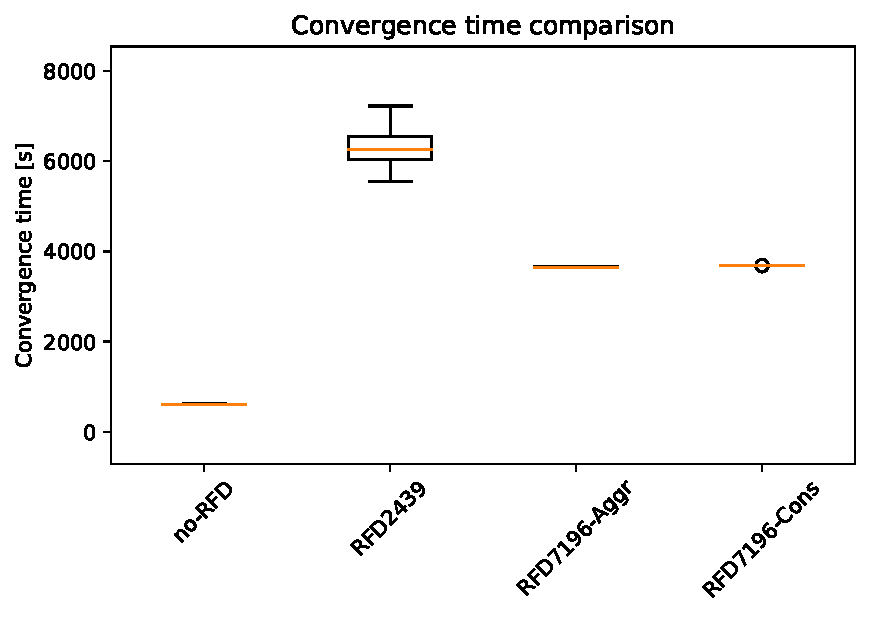
\includegraphics[width=\textwidth]{images/RFD/miceVSelephants/MultiMRAI/0/elephants/cisco_1000MRAI0_rfd_comparison_time_boxplot.pdf}
         \caption{Convergence time respect to the RFD strategy, MRAI=0s}
         \label{fig:1000_RFD_MRAI0_time_elephant}
     \end{subfigure}
     \hfill
     \begin{subfigure}[b]{0.325\textwidth}
         \centering
         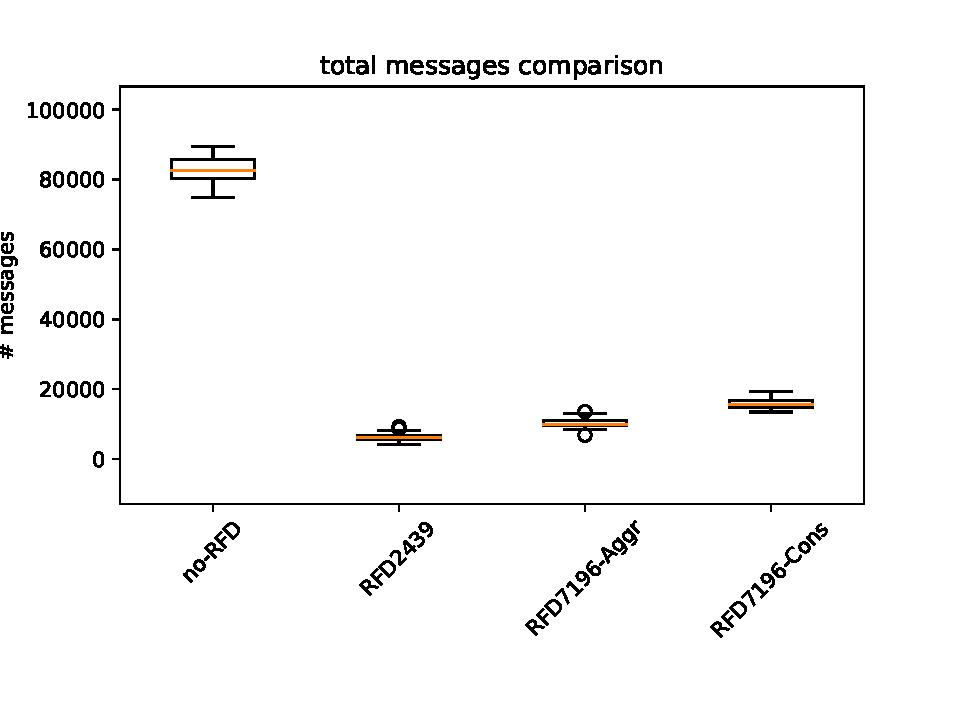
\includegraphics[width=\textwidth]{images/RFD/miceVSelephants/MultiMRAI/0/elephants/cisco_1000MRAI0_rfd_comparison_messages_boxplot.pdf}
         \caption{Number of messages respect to the RFD strategy, MRAI=0s}
         \label{fig:1000_RFD_MRAI0_messages_elephant}
     \end{subfigure}
     \hfill
     \begin{subfigure}[b]{0.325\textwidth}
         \centering
         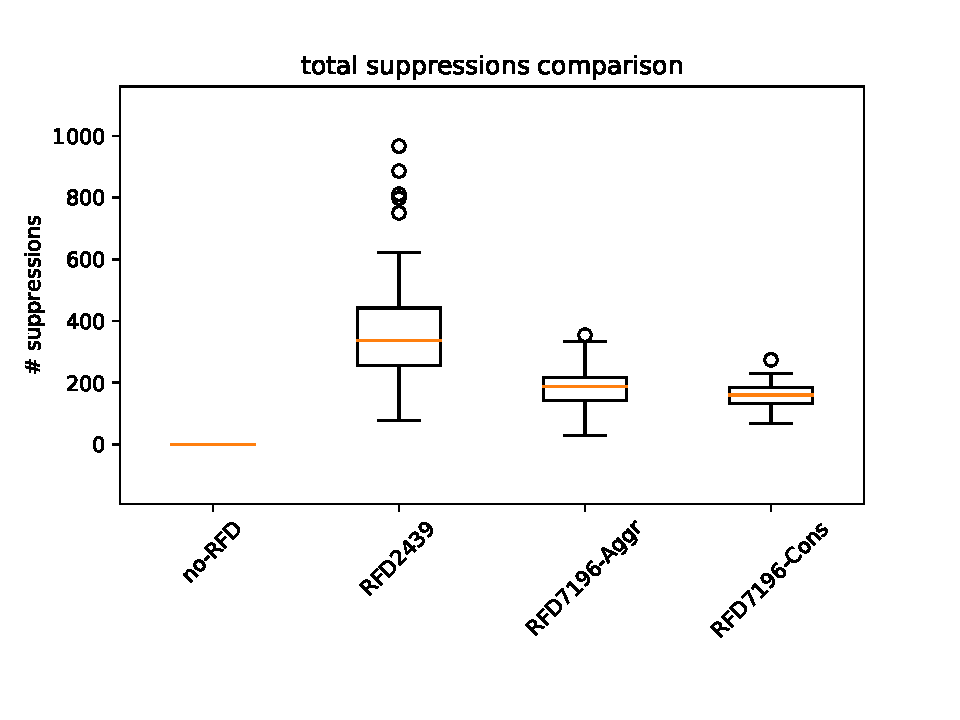
\includegraphics[width=\textwidth]{images/RFD/miceVSelephants/MultiMRAI/0/elephants/cisco_1000MRAI0_rfd_comparison_suppressions_boxplot.pdf}
         \caption{Number of suppressions respect to the RFD strategy, MRAI=0s}
         \label{fig:1000_RFD_MRAI0_suppressions_elephant}
     \end{subfigure}
     \vfill
     \begin{subfigure}[b]{0.325\textwidth}
         \centering
         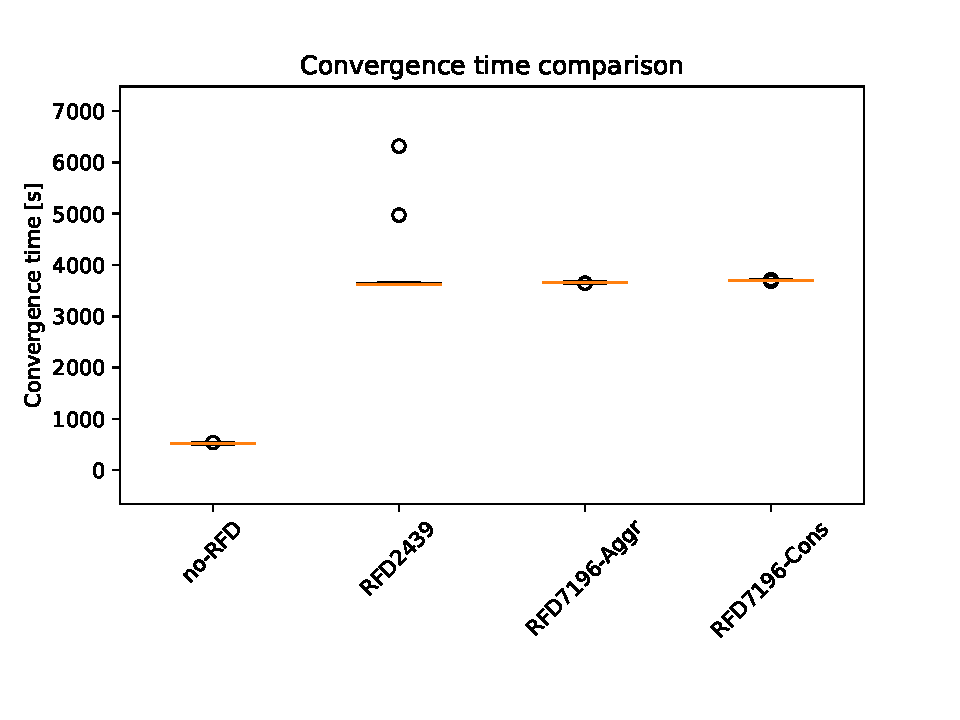
\includegraphics[width=\textwidth]{images/RFD/miceVSelephants/MultiMRAI/15/elephants/cisco_1000MRAI15_rfd_comparison_time_boxplot.pdf}
         \caption{Convergence time respect to the RFD strategy, MRAI=15s}
         \label{fig:1000_RFD_MRAI15_time_elephant}
     \end{subfigure}
     \hfill
     \begin{subfigure}[b]{0.325\textwidth}
         \centering
         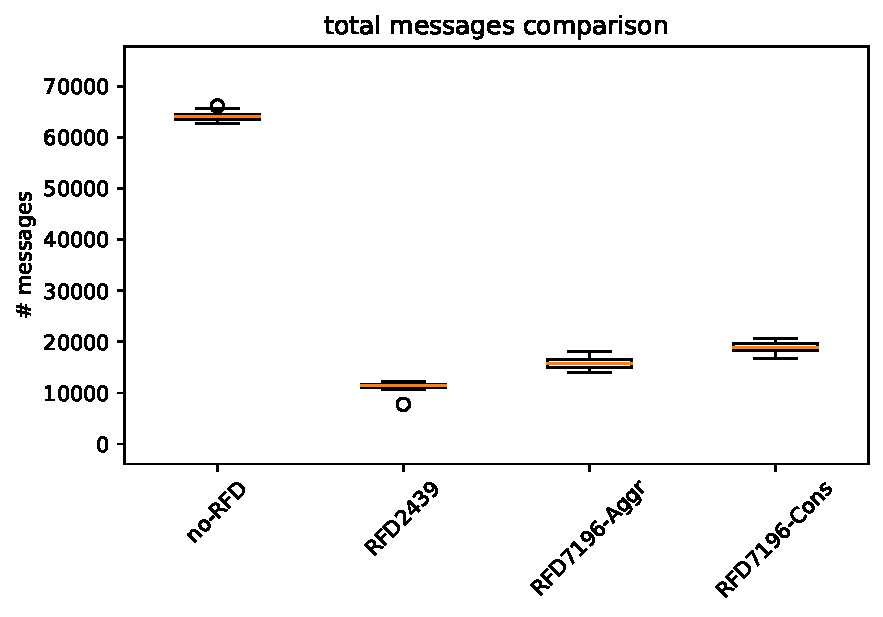
\includegraphics[width=\textwidth]{images/RFD/miceVSelephants/MultiMRAI/15/elephants/cisco_1000MRAI15_rfd_comparison_messages_boxplot.pdf}
         \caption{Number of messages respect to the RFD strategy, MRAI=15s}
         \label{fig:1000_RFD_MRAI15_messages_elephant}
     \end{subfigure}
     \hfill
     \begin{subfigure}[b]{0.325\textwidth}
         \centering
         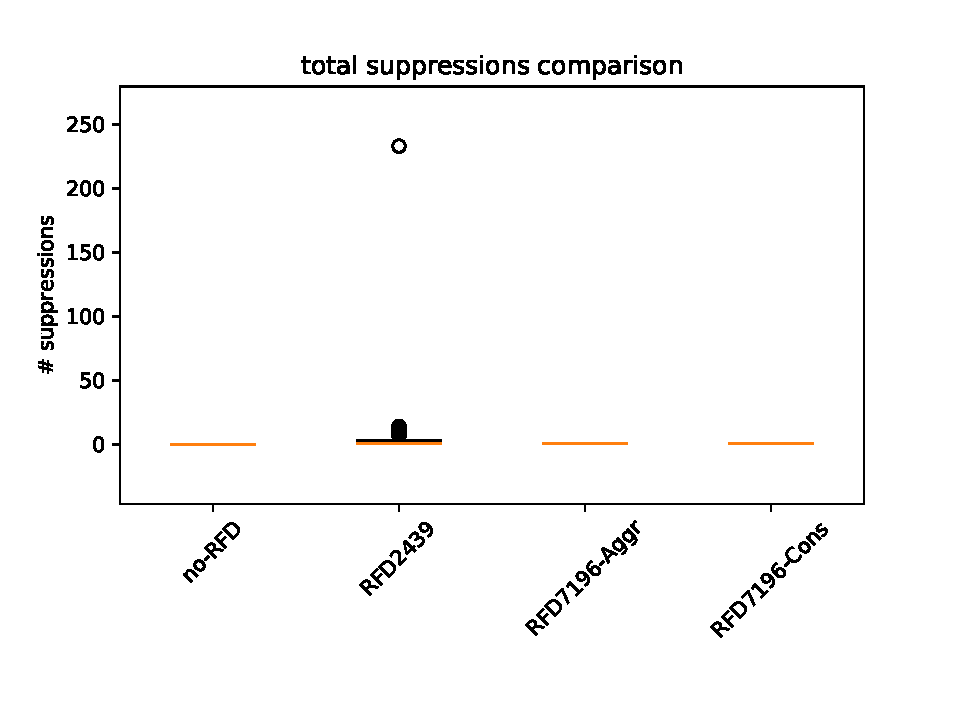
\includegraphics[width=\textwidth]{images/RFD/miceVSelephants/MultiMRAI/15/elephants/cisco_1000MRAI15_rfd_comparison_suppressions_boxplot.pdf}
         \caption{Number of suppressions respect to the RFD strategy, MRAI=15s}
         \label{fig:1000_RFD_MRAI15_suppressions_elephant}
     \end{subfigure}
     \vfill
     \begin{subfigure}[b]{0.325\textwidth}
         \centering
         \includegraphics[width=\textwidth]{images/RFD/miceVSelephants/MultiMRAI/30/elephants/cisco_1000MRAI30_rfd_comparison_time_boxplot.pdf}
         \caption{Convergence time respect to the RFD strategy, MRAI=30s}
         \label{fig:1000_RFD_MRAI30_time_elephant}
     \end{subfigure}
     \hfill
     \begin{subfigure}[b]{0.325\textwidth}
         \centering
         \includegraphics[width=\textwidth]{images/RFD/miceVSelephants/MultiMRAI/30/elephants/cisco_1000MRAI30_rfd_comparison_messages_boxplot.pdf}
         \caption{Number of messages respect to the RFD strategy, MRAI=30s}
         \label{fig:1000_RFD_MRAI30_messages_elephant}
     \end{subfigure}
     \hfill
     \begin{subfigure}[b]{0.325\textwidth}
         \centering
         \includegraphics[width=\textwidth]{images/RFD/miceVSelephants/MultiMRAI/30/elephants/cisco_1000MRAI30_rfd_comparison_suppressions_boxplot.pdf}
         \caption{Number of suppressions respect to the RFD strategy, MRAI=30s}
         \label{fig:1000_RFD_MRAI30_suppressions_elephant}
     \end{subfigure}
     \vfill
     \begin{subfigure}[b]{0.325\textwidth}
         \centering
         \includegraphics[width=\textwidth]{images/RFD/miceVSelephants/MultiMRAI/45/elephants/cisco_1000MRAI45_rfd_comparison_time_boxplot.pdf}
         \caption{Convergence time respect to the RFD strategy, MRAI=45s}
         \label{fig:1000_RFD_MRAI45_time_elephant}
     \end{subfigure}
     \hfill
     \begin{subfigure}[b]{0.325\textwidth}
         \centering
         \includegraphics[width=\textwidth]{images/RFD/miceVSelephants/MultiMRAI/45/elephants/cisco_1000MRAI45_rfd_comparison_messages_boxplot.pdf}
         \caption{Number of messages respect to the RFD strategy, MRAI=30s}
         \label{fig:1000_RFD_MRAI45_messages_elephant}
     \end{subfigure}
     \hfill
     \begin{subfigure}[b]{0.325\textwidth}
         \centering
         \includegraphics[width=\textwidth]{images/RFD/miceVSelephants/MultiMRAI/45/elephants/cisco_1000MRAI45_rfd_comparison_suppressions_boxplot.pdf}
         \caption{Number of suppressions respect to the RFD strategy, MRAI=45s}
         \label{fig:1000_RFD_MRAI45_suppressions_elephant}
     \end{subfigure}
     \vfill
     \begin{subfigure}[b]{0.325\textwidth}
         \centering
         \includegraphics[width=\textwidth]{images/RFD/miceVSelephants/MultiMRAI/60/elephants/cisco_1000MRAI60_rfd_comparison_time_boxplot.pdf}
         \caption{Convergence time respect to the RFD strategy, MRAI=60s}
         \label{fig:1000_RFD_MRAI60_time_elephant}
     \end{subfigure}
     \hfill
     \begin{subfigure}[b]{0.325\textwidth}
         \centering
         \includegraphics[width=\textwidth]{images/RFD/miceVSelephants/MultiMRAI/60/elephants/cisco_1000MRAI60_rfd_comparison_messages_boxplot.pdf}
         \caption{Number of messages respect to the RFD strategy, MRAI=60s}
         \label{fig:1000_RFD_MRAI60_messages_elephant}
     \end{subfigure}
     \hfill
     \begin{subfigure}[b]{0.325\textwidth}
         \centering
         \includegraphics[width=\textwidth]{images/RFD/miceVSelephants/MultiMRAI/60/elephants/cisco_1000MRAI60_rfd_comparison_suppressions_boxplot.pdf}
         \caption{Number of suppressions respect to the RFD strategy, MRAI=60s}
         \label{fig:1000_RFD_MRAI60_suppressions_elephant}
     \end{subfigure}
        \caption{Internet like topology 1000 nodes, random destination, 100 flaps, 3s delay, Network performances}
        \label{fig:1000_RFD_MRAI30_elephant}
\end{figure}

\begin{figure}[H]
     \centering
     \begin{subfigure}[b]{0.325\textwidth}
         \centering
         \includegraphics[width=\textwidth]{images/RFD/miceVSelephants/MultiMRAI/0/elephants/cisco_1000_RFD_nodeConvergence_centVSsup_trend.pdf}
         \caption{RFD 2439 Strategy, \\MRAI=0s}
         \label{fig:1000_2439RFD_centVSsup_elephants_MRAI0}
     \end{subfigure}
     \hfill
     \begin{subfigure}[b]{0.325\textwidth}
         \centering
         \includegraphics[width=\textwidth]{images/RFD/miceVSelephants/MultiMRAI/0/elephants/cisco_1000_RFD_7196_aggressive_nodeConvergence_centVSsup_trend.pdf}
         \caption{RFD 7196 Aggressive Strategy, MRAI=0s}
         \label{fig:1000_7196RFDA_centVSsup_elephants_MRAI0}
     \end{subfigure}
     \hfill
     \begin{subfigure}[b]{0.325\textwidth}
         \centering
         \includegraphics[width=\textwidth]{images/RFD/miceVSelephants/MultiMRAI/0/elephants/cisco_1000_RFD_7196_conservative_nodeConvergence_centVSsup_trend.pdf}
         \caption{RFD 7196 Conservative Strategy, MRAI=0s}
         \label{fig:1000_7196RFDC_centVSsup_elephants_MRAI0}
     \end{subfigure}
     \vfill
     \begin{subfigure}[b]{0.325\textwidth}
         \centering
         \includegraphics[width=\textwidth]{images/RFD/miceVSelephants/MultiMRAI/15/elephants/cisco_1000_RFD_nodeConvergence_centVSsup_trend.pdf}
         \caption{RFD 2439 Strategy, \\MRAI=15s}
         \label{fig:1000_2439RFD_centVSsup_elephants_MRAI15}
     \end{subfigure}
     \hfill
     \begin{subfigure}[b]{0.325\textwidth}
         \centering
         \includegraphics[width=\textwidth]{images/RFD/miceVSelephants/MultiMRAI/15/elephants/cisco_1000_RFD_7196_aggressive_nodeConvergence_centVSsup_trend.pdf}
         \caption{RFD 7196 Aggressive Strategy, MRAI=15s}
         \label{fig:1000_7196RFDA_centVSsup_elephants_MRAI15}
     \end{subfigure}
     \hfill
     \begin{subfigure}[b]{0.325\textwidth}
         \centering
         \includegraphics[width=\textwidth]{images/RFD/miceVSelephants/MultiMRAI/15/elephants/cisco_1000_RFD_7196_conservative_nodeConvergence_centVSsup_trend.pdf}
         \caption{RFD 7196 Conservative Strategy, MRAI=15s}
         \label{fig:1000_7196RFDC_centVSsup_elephants_MRAI15}
     \end{subfigure}
     \vfill
     \begin{subfigure}[b]{0.325\textwidth}
         \centering
         \includegraphics[width=\textwidth]{images/RFD/miceVSelephants/MultiMRAI/30/elephants/cisco_1000_RFD_nodeConvergence_centVSsup_trend.pdf}
         \caption{RFD 2439 Strategy, \\MRAI=30s}
         \label{fig:1000_2439RFD_centVSsup_elephants_MRAI30}
     \end{subfigure}
     \hfill
     \begin{subfigure}[b]{0.325\textwidth}
         \centering
         \includegraphics[width=\textwidth]{images/RFD/miceVSelephants/MultiMRAI/30/elephants/cisco_1000_RFD_7196_aggressive_nodeConvergence_centVSsup_trend.pdf}
         \caption{RFD 7196 Aggressive Strategy, MRAI=30s}
         \label{fig:1000_7196RFDA_centVSsup_elephants_MRAI30}
     \end{subfigure}
     \hfill
     \begin{subfigure}[b]{0.325\textwidth}
         \centering
         \includegraphics[width=\textwidth]{images/RFD/miceVSelephants/MultiMRAI/30/elephants/cisco_1000_RFD_7196_conservative_nodeConvergence_centVSsup_trend.pdf}
         \caption{RFD 7196 Conservative Strategy, MRAI=30s}
         \label{fig:1000_7196RFDC_centVSsup_elephants_MRAI30}
     \end{subfigure}
     \vfill
     \begin{subfigure}[b]{0.325\textwidth}
         \centering
         \includegraphics[width=\textwidth]{images/RFD/miceVSelephants/MultiMRAI/45/elephants/cisco_1000_RFD_nodeConvergence_centVSsup_trend.pdf}
         \caption{RFD 2439 Strategy, \\MRAI=45s}
         \label{fig:1000_2439RFD_centVSsup_elephants_MRAI45}
     \end{subfigure}
     \hfill
     \begin{subfigure}[b]{0.325\textwidth}
         \centering
         \includegraphics[width=\textwidth]{images/RFD/miceVSelephants/MultiMRAI/45/elephants/cisco_1000_RFD_7196_aggressive_nodeConvergence_centVSsup_trend.pdf}
         \caption{RFD 7196 Aggressive Strategy, MRAI=45s}
         \label{fig:1000_7196RFDA_centVSsup_elephants_MRAI45}
     \end{subfigure}
     \hfill
     \begin{subfigure}[b]{0.325\textwidth}
         \centering
         \includegraphics[width=\textwidth]{images/RFD/miceVSelephants/MultiMRAI/45/elephants/cisco_1000_RFD_7196_conservative_nodeConvergence_centVSsup_trend.pdf}
         \caption{RFD 7196 Conservative Strategy, MRAI=45s}
         \label{fig:1000_7196RFDC_centVSsup_elephants_MRAI45}
     \end{subfigure}
     \vfill
     \begin{subfigure}[b]{0.325\textwidth}
         \centering
         \includegraphics[width=\textwidth]{images/RFD/miceVSelephants/MultiMRAI/60/elephants/cisco_1000_RFD_nodeConvergence_centVSsup_trend.pdf}
         \caption{RFD 2439 Strategy, \\MRAI=60s}
         \label{fig:1000_2439RFD_centVSsup_elephants_MRAI60}
     \end{subfigure}
     \hfill
     \begin{subfigure}[b]{0.325\textwidth}
         \centering
         \includegraphics[width=\textwidth]{images/RFD/miceVSelephants/MultiMRAI/60/elephants/cisco_1000_RFD_7196_aggressive_nodeConvergence_centVSsup_trend.pdf}
         \caption{RFD 7196 Aggressive Strategy, MRAI=60s}
         \label{fig:1000_7196RFDA_centVSsup_elephants_MRAI60}
     \end{subfigure}
     \hfill
     \begin{subfigure}[b]{0.325\textwidth}
         \centering
         \includegraphics[width=\textwidth]{images/RFD/miceVSelephants/MultiMRAI/60/elephants/cisco_1000_RFD_7196_conservative_nodeConvergence_centVSsup_trend.pdf}
         \caption{RFD 7196 Conservative Strategy, MRAI=60s}
         \label{fig:1000_7196RFDC_centVSsup_elephants_MRAI60}
     \end{subfigure}
        \caption{Internet like topology 1000 nodes, random destination, 100 flaps, 3s delay, Suppression trend VS avg hop centrality}
        \label{fig:1000_RFD_centVSsup_elephants}
\end{figure}
